%% ECON 282E -- Session 7, Deck A2: Neural Networks as Approximators
%% Sources: AI-ECON Lec03_T2_NN_Concepts.tex, carried WHOLE (16 frames);
%% AI-ECON Lec03_T4 section "Case Study: Curve Fitting and PyTorch";
%% Feng & Miao, "AI for Economists" (Book1), ch.9 sections 9.1-9.2 incl.
%% tab:approx_comparison and tab:activation_guide; Quant_Macro Lec.9 frames
%% 109-114 ("Projection vs Neural Networks", "Basis Function vs Activation
%% Function") -- that file follows Fernandez-Villaverde & Guerron-Quintana and
%% is rewritten here and cited; Quant_Macro Lec.5 "Neural Networks" section,
%% including its "Function Approximation with ReLU" construction.
%% Numbers from tools/figures/s07_numbers.json, keys "activations",
%% "relu_construction", "xor", "param_count", "nn_vs_cheb".
%% Source defects are recorded in slides/SOURCES.md, not on the slides.

%% ECON 282E -- Foundations of Macroeconomics (UC Riverside, Fall 2026)
%% Shared Beamer preamble for every deck in slides/S01 ... slides/S10.
%%
%% Usage (a deck lives in slides/S0X/ and is compiled from that folder):
%%   %% ECON 282E -- Foundations of Macroeconomics (UC Riverside, Fall 2026)
%% Shared Beamer preamble for every deck in slides/S01 ... slides/S10.
%%
%% Usage (a deck lives in slides/S0X/ and is compiled from that folder):
%%   %% ECON 282E -- Foundations of Macroeconomics (UC Riverside, Fall 2026)
%% Shared Beamer preamble for every deck in slides/S01 ... slides/S10.
%%
%% Usage (a deck lives in slides/S0X/ and is compiled from that folder):
%%   \input{../preamble/course_preamble.tex}
%%   \decktitle{1}{A1}{Who I Am \& Why This Course}{September 24, 2026}
%%   \begin{document}
%%   \makedecktitle
%%   ...
%%
%% Adapted from Courses/AI-ECON-2026/source/shared_preamble.tex (Metropolis theme,
%% concept/caution/example/takeaway boxes, \sectiondivider). Changes for this course:
%%   * course title block (\decktitle / \makedecktitle) instead of \makebeamertitle
%%   * \zh{...} typesets Chinese (book titles) under pdflatex via CJKutf8
%%   * researchbox for the "Research in the wild" frames
%%   * section pages off; TikZ libraries and the course map loaded here
%% Build with pdflatex only (two passes); tools/build_slides.py does this for you.

\documentclass[10pt,english,aspectratio=169]{beamer}

\usepackage[T1]{fontenc}
\usepackage{textcomp}
\usepackage[utf8]{inputenc}
\usepackage{babel}
\usepackage{CJKutf8}

\usepackage{amsmath, amssymb, amsthm, graphicx}
\usepackage{booktabs, multirow, tabularx}
\usepackage{tikz}
\usetikzlibrary{positioning,arrows.meta,shapes,calc,fit,backgrounds}
\usepackage{pgfplots}
\pgfplotsset{compat=1.16}
\usepackage[most]{tcolorbox}
\tcbuselibrary{skins, breakable}
\usepackage{listings}
\usepackage{xcolor}

\lstset{
  basicstyle=\ttfamily\small,
  keywordstyle=\color{blue!80!black}\bfseries,
  commentstyle=\color{green!50!black}\itshape,
  stringstyle=\color{orange!80!black},
  backgroundcolor=\color{gray!8},
  frame=single,
  rulecolor=\color{gray!40},
  breaklines=true,
  showstringspaces=false,
  numbers=none,
}

\usetheme{metropolis}
\usefonttheme{professionalfonts}
\metroset{sectionpage=none}

\definecolor{LightGray}{RGB}{230,230,230}
\definecolor{RedTitle}{RGB}{0,0,200}
\definecolor{VeryLightGray}{RGB}{245,245,245}
\definecolor{DarkText}{RGB}{0,0,0}
\definecolor{UCRBlue}{RGB}{0,45,106}
\definecolor{UCRGold}{RGB}{241,171,0}

% Stage colours of the course arc (used by the course map and elsewhere)
\colorlet{StageTrunk}{blue!12}
\colorlet{StageBranch}{cyan!14}
\colorlet{StageMachine}{gray!18}
\colorlet{StageWall}{red!14}
\colorlet{StageTools}{orange!20}
\colorlet{StageData}{green!16}
\colorlet{StageAgents}{violet!14}

\hypersetup{bookmarks=false,breaklinks=true,pdfborder={0 0 0},colorlinks=true,
  linkcolor=DarkText,urlcolor=RedTitle}

\setbeamercolor{background canvas}{bg=white}
\setbeamercolor{title}{fg=RedTitle}
\setbeamercolor{frametitle}{bg=VeryLightGray,fg=DarkText}
\setbeamercolor{normal text}{fg=DarkText}
\setbeamercolor{alerted text}{fg=RedTitle}
\setbeamersize{text margin left=5mm, text margin right=5mm}
\addtobeamertemplate{frametitle}{}{\vspace{-0.5em}}

\setbeamertemplate{navigation symbols}{}
\setbeamertemplate{footline}{%
  \hspace{5mm}{\usebeamerfont{page number in head/foot}\color{black!45}%
  ECON 282E \,$\cdot$\, \insertshortdeck}\hfill%
  \usebeamercolor[fg]{page number in head/foot}%
  \usebeamerfont{page number in head/foot}%
  \insertframenumber\,/\,\inserttotalframenumber\kern1em\vskip2pt%
}

% ---------------------------------------------------------------------------
% Chinese text under pdflatex (book titles etc.)
\newcommand{\zh}[1]{\begin{CJK*}{UTF8}{gbsn}#1\end{CJK*}}

% ---------------------------------------------------------------------------
% Deck title block
%   \decktitle{session}{deck id}{title}{date}
\newcommand{\insertshortdeck}{}
\newcommand{\decksession}{}
\newcommand{\deckid}{}
\newcommand{\decktitletext}{}
\newcommand{\deckdate}{}
\newcommand{\decktitle}[4]{%
  \renewcommand{\decksession}{#1}%
  \renewcommand{\deckid}{#2}%
  \renewcommand{\decktitletext}{#3}%
  \renewcommand{\deckdate}{#4}%
  \renewcommand{\insertshortdeck}{Session #1 \,$\cdot$\, Deck #1.#2}%
  \title{#3}%
  \author{Zhigang Feng}%
  \date{#4}%
}
\newcommand{\makedecktitle}{%
  \begin{frame}[plain,noframenumbering]
    \begin{tikzpicture}[remember picture,overlay]
      \fill[UCRBlue] (current page.north west) rectangle ([yshift=-0.55cm]current page.north east);
      \fill[UCRGold] ([yshift=-0.55cm]current page.north west) rectangle ([yshift=-0.62cm]current page.north east);
      \node[anchor=west, text=white, font=\small\bfseries] at ([xshift=5mm,yshift=-0.275cm]current page.north west)
        {ECON 282E \,$\cdot$\, Foundations of Macroeconomics};
      \node[anchor=east, text=white, font=\small] at ([xshift=-5mm,yshift=-0.275cm]current page.north east)
        {UC Riverside \,$\cdot$\, Fall 2026};
    \end{tikzpicture}
    \vspace*{1.1cm}
    {\usebeamerfont{title}\color{black!55}\large Session \decksession\ \,$\cdot$\, Deck \decksession.\deckid\par}
    \vspace{0.25cm}
    {\usebeamerfont{title}\color{RedTitle}\LARGE\bfseries \decktitletext\par}
    \vspace{0.7cm}
    {\large Zhigang Feng\par}
    \vspace{0.15cm}
    {\color{black!65}\deckdate\par}
    \vfill
    {\footnotesize\itshape\color{black!55}Build it on paper $\;\to\;$ solve it on the machine $\;\to\;$ push it to the frontier with AI\par}
  \end{frame}}

% ---------------------------------------------------------------------------
% Section divider (plain frame, not counted)
\newcommand{\sectiondivider}[2]{%
\begin{frame}[plain,noframenumbering]
\begin{center}
\vfill
{\Large\textbf{#1}\par}
\vspace{0.35cm}
{\normalsize #2\par}
\vfill
\end{center}
\end{frame}
}

% ---------------------------------------------------------------------------
% Boxes
\newtcolorbox{conceptbox}[1][]{colback=blue!3, colframe=RedTitle!55, boxrule=0.35mm,
  arc=1mm, left=2mm, right=2mm, top=1mm, bottom=1mm, #1}
\newtcolorbox{cautionbox}[1][]{colback=red!3, colframe=red!50!black, boxrule=0.35mm,
  arc=1mm, left=2mm, right=2mm, top=1mm, bottom=1mm, #1}
\newtcolorbox{examplebox}[1][]{colback=green!3, colframe=green!45!black, boxrule=0.35mm,
  arc=1mm, left=2mm, right=2mm, top=1mm, bottom=1mm, #1}
\newtcolorbox{takeawaybox}[1][]{colback=VeryLightGray, colframe=RedTitle!55, boxrule=0.35mm,
  arc=1mm, left=2mm, right=2mm, top=1mm, bottom=1mm, #1}
\newtcolorbox{researchbox}[1][]{enhanced, colback=violet!4, colframe=violet!60!black,
  boxrule=0.35mm, arc=1mm, left=2mm, right=2mm, top=1mm, bottom=1mm,
  fonttitle=\bfseries\small, title={Research in the wild}, #1}

\newcommand{\compacttables}{\renewcommand{\arraystretch}{1.15}}
\newcommand{\src}[1]{{\tiny\color{black!55}#1}}

% ---------------------------------------------------------------------------
\input{../preamble/course_map.tex}

%%   \decktitle{1}{A1}{Who I Am \& Why This Course}{September 24, 2026}
%%   \begin{document}
%%   \makedecktitle
%%   ...
%%
%% Adapted from Courses/AI-ECON-2026/source/shared_preamble.tex (Metropolis theme,
%% concept/caution/example/takeaway boxes, \sectiondivider). Changes for this course:
%%   * course title block (\decktitle / \makedecktitle) instead of \makebeamertitle
%%   * \zh{...} typesets Chinese (book titles) under pdflatex via CJKutf8
%%   * researchbox for the "Research in the wild" frames
%%   * section pages off; TikZ libraries and the course map loaded here
%% Build with pdflatex only (two passes); tools/build_slides.py does this for you.

\documentclass[10pt,english,aspectratio=169]{beamer}

\usepackage[T1]{fontenc}
\usepackage{textcomp}
\usepackage[utf8]{inputenc}
\usepackage{babel}
\usepackage{CJKutf8}

\usepackage{amsmath, amssymb, amsthm, graphicx}
\usepackage{booktabs, multirow, tabularx}
\usepackage{tikz}
\usetikzlibrary{positioning,arrows.meta,shapes,calc,fit,backgrounds}
\usepackage{pgfplots}
\pgfplotsset{compat=1.16}
\usepackage[most]{tcolorbox}
\tcbuselibrary{skins, breakable}
\usepackage{listings}
\usepackage{xcolor}

\lstset{
  basicstyle=\ttfamily\small,
  keywordstyle=\color{blue!80!black}\bfseries,
  commentstyle=\color{green!50!black}\itshape,
  stringstyle=\color{orange!80!black},
  backgroundcolor=\color{gray!8},
  frame=single,
  rulecolor=\color{gray!40},
  breaklines=true,
  showstringspaces=false,
  numbers=none,
}

\usetheme{metropolis}
\usefonttheme{professionalfonts}
\metroset{sectionpage=none}

\definecolor{LightGray}{RGB}{230,230,230}
\definecolor{RedTitle}{RGB}{0,0,200}
\definecolor{VeryLightGray}{RGB}{245,245,245}
\definecolor{DarkText}{RGB}{0,0,0}
\definecolor{UCRBlue}{RGB}{0,45,106}
\definecolor{UCRGold}{RGB}{241,171,0}

% Stage colours of the course arc (used by the course map and elsewhere)
\colorlet{StageTrunk}{blue!12}
\colorlet{StageBranch}{cyan!14}
\colorlet{StageMachine}{gray!18}
\colorlet{StageWall}{red!14}
\colorlet{StageTools}{orange!20}
\colorlet{StageData}{green!16}
\colorlet{StageAgents}{violet!14}

\hypersetup{bookmarks=false,breaklinks=true,pdfborder={0 0 0},colorlinks=true,
  linkcolor=DarkText,urlcolor=RedTitle}

\setbeamercolor{background canvas}{bg=white}
\setbeamercolor{title}{fg=RedTitle}
\setbeamercolor{frametitle}{bg=VeryLightGray,fg=DarkText}
\setbeamercolor{normal text}{fg=DarkText}
\setbeamercolor{alerted text}{fg=RedTitle}
\setbeamersize{text margin left=5mm, text margin right=5mm}
\addtobeamertemplate{frametitle}{}{\vspace{-0.5em}}

\setbeamertemplate{navigation symbols}{}
\setbeamertemplate{footline}{%
  \hspace{5mm}{\usebeamerfont{page number in head/foot}\color{black!45}%
  ECON 282E \,$\cdot$\, \insertshortdeck}\hfill%
  \usebeamercolor[fg]{page number in head/foot}%
  \usebeamerfont{page number in head/foot}%
  \insertframenumber\,/\,\inserttotalframenumber\kern1em\vskip2pt%
}

% ---------------------------------------------------------------------------
% Chinese text under pdflatex (book titles etc.)
\newcommand{\zh}[1]{\begin{CJK*}{UTF8}{gbsn}#1\end{CJK*}}

% ---------------------------------------------------------------------------
% Deck title block
%   \decktitle{session}{deck id}{title}{date}
\newcommand{\insertshortdeck}{}
\newcommand{\decksession}{}
\newcommand{\deckid}{}
\newcommand{\decktitletext}{}
\newcommand{\deckdate}{}
\newcommand{\decktitle}[4]{%
  \renewcommand{\decksession}{#1}%
  \renewcommand{\deckid}{#2}%
  \renewcommand{\decktitletext}{#3}%
  \renewcommand{\deckdate}{#4}%
  \renewcommand{\insertshortdeck}{Session #1 \,$\cdot$\, Deck #1.#2}%
  \title{#3}%
  \author{Zhigang Feng}%
  \date{#4}%
}
\newcommand{\makedecktitle}{%
  \begin{frame}[plain,noframenumbering]
    \begin{tikzpicture}[remember picture,overlay]
      \fill[UCRBlue] (current page.north west) rectangle ([yshift=-0.55cm]current page.north east);
      \fill[UCRGold] ([yshift=-0.55cm]current page.north west) rectangle ([yshift=-0.62cm]current page.north east);
      \node[anchor=west, text=white, font=\small\bfseries] at ([xshift=5mm,yshift=-0.275cm]current page.north west)
        {ECON 282E \,$\cdot$\, Foundations of Macroeconomics};
      \node[anchor=east, text=white, font=\small] at ([xshift=-5mm,yshift=-0.275cm]current page.north east)
        {UC Riverside \,$\cdot$\, Fall 2026};
    \end{tikzpicture}
    \vspace*{1.1cm}
    {\usebeamerfont{title}\color{black!55}\large Session \decksession\ \,$\cdot$\, Deck \decksession.\deckid\par}
    \vspace{0.25cm}
    {\usebeamerfont{title}\color{RedTitle}\LARGE\bfseries \decktitletext\par}
    \vspace{0.7cm}
    {\large Zhigang Feng\par}
    \vspace{0.15cm}
    {\color{black!65}\deckdate\par}
    \vfill
    {\footnotesize\itshape\color{black!55}Build it on paper $\;\to\;$ solve it on the machine $\;\to\;$ push it to the frontier with AI\par}
  \end{frame}}

% ---------------------------------------------------------------------------
% Section divider (plain frame, not counted)
\newcommand{\sectiondivider}[2]{%
\begin{frame}[plain,noframenumbering]
\begin{center}
\vfill
{\Large\textbf{#1}\par}
\vspace{0.35cm}
{\normalsize #2\par}
\vfill
\end{center}
\end{frame}
}

% ---------------------------------------------------------------------------
% Boxes
\newtcolorbox{conceptbox}[1][]{colback=blue!3, colframe=RedTitle!55, boxrule=0.35mm,
  arc=1mm, left=2mm, right=2mm, top=1mm, bottom=1mm, #1}
\newtcolorbox{cautionbox}[1][]{colback=red!3, colframe=red!50!black, boxrule=0.35mm,
  arc=1mm, left=2mm, right=2mm, top=1mm, bottom=1mm, #1}
\newtcolorbox{examplebox}[1][]{colback=green!3, colframe=green!45!black, boxrule=0.35mm,
  arc=1mm, left=2mm, right=2mm, top=1mm, bottom=1mm, #1}
\newtcolorbox{takeawaybox}[1][]{colback=VeryLightGray, colframe=RedTitle!55, boxrule=0.35mm,
  arc=1mm, left=2mm, right=2mm, top=1mm, bottom=1mm, #1}
\newtcolorbox{researchbox}[1][]{enhanced, colback=violet!4, colframe=violet!60!black,
  boxrule=0.35mm, arc=1mm, left=2mm, right=2mm, top=1mm, bottom=1mm,
  fonttitle=\bfseries\small, title={Research in the wild}, #1}

\newcommand{\compacttables}{\renewcommand{\arraystretch}{1.15}}
\newcommand{\src}[1]{{\tiny\color{black!55}#1}}

% ---------------------------------------------------------------------------
%% Course map: the recurring "you are here" slide for ECON 282E.
%% Loaded by course_preamble.tex. Pattern follows AI-ECON-2026 lec01_map.tex, but the map
%% shows the whole ten-session course rather than one lecture.
%%
%%   \CourseMap{s}{label}   s = 1..10 highlights session s and prints "you are here: label"
%%                          (e.g. \CourseMap{1}{1.A2}); earlier sessions get a check mark.
%%   \CourseMap{0}{}        full overview, nothing highlighted.
%%
%% Note: TikZ option lists are comma-split before TeX conditionals run, so every \ifnum
%% below sits outside [...] option lists.

\newcommand{\CourseMap}[2]{%
\begin{center}
\begin{tikzpicture}[
    sess/.style={rectangle, rounded corners=2pt, draw=black!45, minimum width=1.34cm,
        minimum height=1.12cm, text width=1.26cm, align=center, inner sep=1pt},
    stage/.style={font=\tiny\bfseries, text=black!70},
]
  \foreach \i/\d/\t/\c in {%
      1/Sep 24/Intro \\ Growth/StageTrunk,
      2/Oct 1/HA $\cdot$ OLG \\ Policy/StageBranch,
      3/Oct 8/Num.\ DP \\ Python/StageMachine,
      4/Oct 15/Numerics \\ I/StageMachine,
      5/Oct 22/Numerics \\ II/StageMachine,
      6/Oct 29/The wall \\ \textbf{Midterm}/StageWall,
      7/Nov 5/ML \\ Deep nets/StageTools,
      8/Nov 12/RL \\ HA $+$ DL/StageTools,
      9/Nov 19/Text \\ LLMs/StageData,
      10/Dec 3/Agents \\ \textbf{Projects}/StageAgents} {
    \node[sess, fill=\c] (n\i) at ({1.46*(\i-1)}, 0)
      {{\scriptsize\bfseries S\i}\\[-1pt]{\tiny\color{black!60}\d}\\[1pt]{\tiny \t}};
    \ifnum\i<#1
      \node[font=\scriptsize, text=green!45!black] at ([xshift=-2.5mm,yshift=-2.2mm]n\i.north east) {$\checkmark$};
    \fi
    \ifnum\i=#1
      \draw[RedTitle, very thick, rounded corners=2pt]
        ([xshift=-0.6mm,yshift=-0.6mm]n\i.south west) rectangle ([xshift=0.6mm,yshift=0.6mm]n\i.north east);
      % keep the label inside the picture at both ends of the row
      \ifnum\i<3
        \node[font=\scriptsize\bfseries, text=RedTitle, anchor=south west] at ([yshift=1.2mm]n\i.north west)
          {$\blacktriangledown$\,you are here: #2};
      \else\ifnum\i>8
        \node[font=\scriptsize\bfseries, text=RedTitle, anchor=south east] at ([yshift=1.2mm]n\i.north east)
          {you are here: #2\,$\blacktriangledown$};
      \else
        \node[font=\scriptsize\bfseries, text=RedTitle, anchor=south] at ([yshift=1.2mm]n\i.north)
          {you are here: #2\,$\blacktriangledown$};
      \fi\fi
    \fi
  }
  % stage band under the sessions
  \foreach \a/\b/\lab/\c in {1/1/trunk/StageTrunk, 2/2/branches/StageBranch,
      3/5/the machine $\cdot$ classical methods/StageMachine, 6/6/the wall/StageWall,
      7/8/new tools/StageTools, 9/9/new data/StageData, 10/10/colleagues/StageAgents} {
    \fill[\c] ([yshift=-1.5mm]n\a.south west) rectangle ([yshift=-4.6mm]n\b.south east);
    \path ([yshift=-1.5mm]n\a.south west) -- ([yshift=-4.6mm]n\b.south east)
      node[midway, stage] {\lab};
  }
  \node[font=\footnotesize\itshape, text=black!70] at ([yshift=-9.5mm]$(n1.south)!0.5!(n10.south)$)
    {Build it on paper $\;\to\;$ solve it on the machine $\;\to\;$ push it to the frontier with AI};
\end{tikzpicture}
\end{center}
}


%%   \decktitle{1}{A1}{Who I Am \& Why This Course}{September 24, 2026}
%%   \begin{document}
%%   \makedecktitle
%%   ...
%%
%% Adapted from Courses/AI-ECON-2026/source/shared_preamble.tex (Metropolis theme,
%% concept/caution/example/takeaway boxes, \sectiondivider). Changes for this course:
%%   * course title block (\decktitle / \makedecktitle) instead of \makebeamertitle
%%   * \zh{...} typesets Chinese (book titles) under pdflatex via CJKutf8
%%   * researchbox for the "Research in the wild" frames
%%   * section pages off; TikZ libraries and the course map loaded here
%% Build with pdflatex only (two passes); tools/build_slides.py does this for you.

\documentclass[10pt,english,aspectratio=169]{beamer}

\usepackage[T1]{fontenc}
\usepackage{textcomp}
\usepackage[utf8]{inputenc}
\usepackage{babel}
\usepackage{CJKutf8}

\usepackage{amsmath, amssymb, amsthm, graphicx}
\usepackage{booktabs, multirow, tabularx}
\usepackage{tikz}
\usetikzlibrary{positioning,arrows.meta,shapes,calc,fit,backgrounds}
\usepackage{pgfplots}
\pgfplotsset{compat=1.16}
\usepackage[most]{tcolorbox}
\tcbuselibrary{skins, breakable}
\usepackage{listings}
\usepackage{xcolor}

\lstset{
  basicstyle=\ttfamily\small,
  keywordstyle=\color{blue!80!black}\bfseries,
  commentstyle=\color{green!50!black}\itshape,
  stringstyle=\color{orange!80!black},
  backgroundcolor=\color{gray!8},
  frame=single,
  rulecolor=\color{gray!40},
  breaklines=true,
  showstringspaces=false,
  numbers=none,
}

\usetheme{metropolis}
\usefonttheme{professionalfonts}
\metroset{sectionpage=none}

\definecolor{LightGray}{RGB}{230,230,230}
\definecolor{RedTitle}{RGB}{0,0,200}
\definecolor{VeryLightGray}{RGB}{245,245,245}
\definecolor{DarkText}{RGB}{0,0,0}
\definecolor{UCRBlue}{RGB}{0,45,106}
\definecolor{UCRGold}{RGB}{241,171,0}

% Stage colours of the course arc (used by the course map and elsewhere)
\colorlet{StageTrunk}{blue!12}
\colorlet{StageBranch}{cyan!14}
\colorlet{StageMachine}{gray!18}
\colorlet{StageWall}{red!14}
\colorlet{StageTools}{orange!20}
\colorlet{StageData}{green!16}
\colorlet{StageAgents}{violet!14}

\hypersetup{bookmarks=false,breaklinks=true,pdfborder={0 0 0},colorlinks=true,
  linkcolor=DarkText,urlcolor=RedTitle}

\setbeamercolor{background canvas}{bg=white}
\setbeamercolor{title}{fg=RedTitle}
\setbeamercolor{frametitle}{bg=VeryLightGray,fg=DarkText}
\setbeamercolor{normal text}{fg=DarkText}
\setbeamercolor{alerted text}{fg=RedTitle}
\setbeamersize{text margin left=5mm, text margin right=5mm}
\addtobeamertemplate{frametitle}{}{\vspace{-0.5em}}

\setbeamertemplate{navigation symbols}{}
\setbeamertemplate{footline}{%
  \hspace{5mm}{\usebeamerfont{page number in head/foot}\color{black!45}%
  ECON 282E \,$\cdot$\, \insertshortdeck}\hfill%
  \usebeamercolor[fg]{page number in head/foot}%
  \usebeamerfont{page number in head/foot}%
  \insertframenumber\,/\,\inserttotalframenumber\kern1em\vskip2pt%
}

% ---------------------------------------------------------------------------
% Chinese text under pdflatex (book titles etc.)
\newcommand{\zh}[1]{\begin{CJK*}{UTF8}{gbsn}#1\end{CJK*}}

% ---------------------------------------------------------------------------
% Deck title block
%   \decktitle{session}{deck id}{title}{date}
\newcommand{\insertshortdeck}{}
\newcommand{\decksession}{}
\newcommand{\deckid}{}
\newcommand{\decktitletext}{}
\newcommand{\deckdate}{}
\newcommand{\decktitle}[4]{%
  \renewcommand{\decksession}{#1}%
  \renewcommand{\deckid}{#2}%
  \renewcommand{\decktitletext}{#3}%
  \renewcommand{\deckdate}{#4}%
  \renewcommand{\insertshortdeck}{Session #1 \,$\cdot$\, Deck #1.#2}%
  \title{#3}%
  \author{Zhigang Feng}%
  \date{#4}%
}
\newcommand{\makedecktitle}{%
  \begin{frame}[plain,noframenumbering]
    \begin{tikzpicture}[remember picture,overlay]
      \fill[UCRBlue] (current page.north west) rectangle ([yshift=-0.55cm]current page.north east);
      \fill[UCRGold] ([yshift=-0.55cm]current page.north west) rectangle ([yshift=-0.62cm]current page.north east);
      \node[anchor=west, text=white, font=\small\bfseries] at ([xshift=5mm,yshift=-0.275cm]current page.north west)
        {ECON 282E \,$\cdot$\, Foundations of Macroeconomics};
      \node[anchor=east, text=white, font=\small] at ([xshift=-5mm,yshift=-0.275cm]current page.north east)
        {UC Riverside \,$\cdot$\, Fall 2026};
    \end{tikzpicture}
    \vspace*{1.1cm}
    {\usebeamerfont{title}\color{black!55}\large Session \decksession\ \,$\cdot$\, Deck \decksession.\deckid\par}
    \vspace{0.25cm}
    {\usebeamerfont{title}\color{RedTitle}\LARGE\bfseries \decktitletext\par}
    \vspace{0.7cm}
    {\large Zhigang Feng\par}
    \vspace{0.15cm}
    {\color{black!65}\deckdate\par}
    \vfill
    {\footnotesize\itshape\color{black!55}Build it on paper $\;\to\;$ solve it on the machine $\;\to\;$ push it to the frontier with AI\par}
  \end{frame}}

% ---------------------------------------------------------------------------
% Section divider (plain frame, not counted)
\newcommand{\sectiondivider}[2]{%
\begin{frame}[plain,noframenumbering]
\begin{center}
\vfill
{\Large\textbf{#1}\par}
\vspace{0.35cm}
{\normalsize #2\par}
\vfill
\end{center}
\end{frame}
}

% ---------------------------------------------------------------------------
% Boxes
\newtcolorbox{conceptbox}[1][]{colback=blue!3, colframe=RedTitle!55, boxrule=0.35mm,
  arc=1mm, left=2mm, right=2mm, top=1mm, bottom=1mm, #1}
\newtcolorbox{cautionbox}[1][]{colback=red!3, colframe=red!50!black, boxrule=0.35mm,
  arc=1mm, left=2mm, right=2mm, top=1mm, bottom=1mm, #1}
\newtcolorbox{examplebox}[1][]{colback=green!3, colframe=green!45!black, boxrule=0.35mm,
  arc=1mm, left=2mm, right=2mm, top=1mm, bottom=1mm, #1}
\newtcolorbox{takeawaybox}[1][]{colback=VeryLightGray, colframe=RedTitle!55, boxrule=0.35mm,
  arc=1mm, left=2mm, right=2mm, top=1mm, bottom=1mm, #1}
\newtcolorbox{researchbox}[1][]{enhanced, colback=violet!4, colframe=violet!60!black,
  boxrule=0.35mm, arc=1mm, left=2mm, right=2mm, top=1mm, bottom=1mm,
  fonttitle=\bfseries\small, title={Research in the wild}, #1}

\newcommand{\compacttables}{\renewcommand{\arraystretch}{1.15}}
\newcommand{\src}[1]{{\tiny\color{black!55}#1}}

% ---------------------------------------------------------------------------
%% Course map: the recurring "you are here" slide for ECON 282E.
%% Loaded by course_preamble.tex. Pattern follows AI-ECON-2026 lec01_map.tex, but the map
%% shows the whole ten-session course rather than one lecture.
%%
%%   \CourseMap{s}{label}   s = 1..10 highlights session s and prints "you are here: label"
%%                          (e.g. \CourseMap{1}{1.A2}); earlier sessions get a check mark.
%%   \CourseMap{0}{}        full overview, nothing highlighted.
%%
%% Note: TikZ option lists are comma-split before TeX conditionals run, so every \ifnum
%% below sits outside [...] option lists.

\newcommand{\CourseMap}[2]{%
\begin{center}
\begin{tikzpicture}[
    sess/.style={rectangle, rounded corners=2pt, draw=black!45, minimum width=1.34cm,
        minimum height=1.12cm, text width=1.26cm, align=center, inner sep=1pt},
    stage/.style={font=\tiny\bfseries, text=black!70},
]
  \foreach \i/\d/\t/\c in {%
      1/Sep 24/Intro \\ Growth/StageTrunk,
      2/Oct 1/HA $\cdot$ OLG \\ Policy/StageBranch,
      3/Oct 8/Num.\ DP \\ Python/StageMachine,
      4/Oct 15/Numerics \\ I/StageMachine,
      5/Oct 22/Numerics \\ II/StageMachine,
      6/Oct 29/The wall \\ \textbf{Midterm}/StageWall,
      7/Nov 5/ML \\ Deep nets/StageTools,
      8/Nov 12/RL \\ HA $+$ DL/StageTools,
      9/Nov 19/Text \\ LLMs/StageData,
      10/Dec 3/Agents \\ \textbf{Projects}/StageAgents} {
    \node[sess, fill=\c] (n\i) at ({1.46*(\i-1)}, 0)
      {{\scriptsize\bfseries S\i}\\[-1pt]{\tiny\color{black!60}\d}\\[1pt]{\tiny \t}};
    \ifnum\i<#1
      \node[font=\scriptsize, text=green!45!black] at ([xshift=-2.5mm,yshift=-2.2mm]n\i.north east) {$\checkmark$};
    \fi
    \ifnum\i=#1
      \draw[RedTitle, very thick, rounded corners=2pt]
        ([xshift=-0.6mm,yshift=-0.6mm]n\i.south west) rectangle ([xshift=0.6mm,yshift=0.6mm]n\i.north east);
      % keep the label inside the picture at both ends of the row
      \ifnum\i<3
        \node[font=\scriptsize\bfseries, text=RedTitle, anchor=south west] at ([yshift=1.2mm]n\i.north west)
          {$\blacktriangledown$\,you are here: #2};
      \else\ifnum\i>8
        \node[font=\scriptsize\bfseries, text=RedTitle, anchor=south east] at ([yshift=1.2mm]n\i.north east)
          {you are here: #2\,$\blacktriangledown$};
      \else
        \node[font=\scriptsize\bfseries, text=RedTitle, anchor=south] at ([yshift=1.2mm]n\i.north)
          {you are here: #2\,$\blacktriangledown$};
      \fi\fi
    \fi
  }
  % stage band under the sessions
  \foreach \a/\b/\lab/\c in {1/1/trunk/StageTrunk, 2/2/branches/StageBranch,
      3/5/the machine $\cdot$ classical methods/StageMachine, 6/6/the wall/StageWall,
      7/8/new tools/StageTools, 9/9/new data/StageData, 10/10/colleagues/StageAgents} {
    \fill[\c] ([yshift=-1.5mm]n\a.south west) rectangle ([yshift=-4.6mm]n\b.south east);
    \path ([yshift=-1.5mm]n\a.south west) -- ([yshift=-4.6mm]n\b.south east)
      node[midway, stage] {\lab};
  }
  \node[font=\footnotesize\itshape, text=black!70] at ([yshift=-9.5mm]$(n1.south)!0.5!(n10.south)$)
    {Build it on paper $\;\to\;$ solve it on the machine $\;\to\;$ push it to the frontier with AI};
\end{tikzpicture}
\end{center}
}


\graphicspath{{./figures/}}

%% Deck-local: the shared preamble is never edited (its md5 marks every deck stale).
\newcommand{\repo}[2]{\href{https://github.com/vonzhg/Macro-2026Fall/blob/main/#1}{\texttt{#2}}}

\decktitle{7}{A2}{Neural Networks as Approximators}{Thursday, November 5, 2026}

\begin{document}

\makedecktitle

%=============================================================================
\begin{frame}{Where We Are}
\CourseMap{7}{7.A2}
\vspace{-1mm}
\begin{center}
\small \textbf{Block A:} 7.A1 ML for macroeconomists $\;\cdot\;$ \textbf{7.A2} nets as approximators $\;\cdot\;$ 7.A3 training $\;\cdot\;$ 7.A4 architecture.
\end{center}
\end{frame}

%=============================================================================
\begin{frame}{What We Are Building, and What We Will Ask of It}
\begin{columns}[T]
\begin{column}{0.55\textwidth}
\small
7.A1 ended on a sentence: a network is $\mathcal{N}(x;\theta)$, and the basis functions are built out of $\theta$ rather than chosen in advance.
\medskip

This deck makes that concrete and then interrogates it, in that order:
\begin{enumerate}\small\setlength{\itemsep}{1.1mm}
  \item \textbf{the object} --- neuron, layer, composition, and why the nonlinearity between layers is load-bearing;
  \item \textbf{the construction} --- build an approximation out of kinks, by hand, and watch what changes when the kinks are allowed to move;
  \item \textbf{the theorems} --- what universal approximation promises, what Barron's rate promises, and what neither of them promises.
\end{enumerate}
\end{column}
\begin{column}{0.42\textwidth}
\begin{conceptbox}[title=\textbf{The comparison to keep}]\small
5.B2 asked ``which basis?'' and answered with orthogonality, conditioning, and a convergence rate you could bound.
\medskip
Everything in this deck is the same question asked of an object that will not give you any of those three --- and the honest accounting of what you get instead.
\end{conceptbox}
\end{column}
\end{columns}
\end{frame}

%=============================================================================
\begin{frame}{A Neuron Is a Regression with a Nonlinear Output}
\begin{columns}[T]
\begin{column}{0.52\textwidth}
\small
One unit does two things. First a \textbf{net input},
\[
  z=\mathbf{w}^{\top}\mathbf{x}+b ,
\]
which you have written a thousand times --- it is a linear index. Then an \textbf{activation},
\[
  a=\sigma(z).
\]
\medskip

That is the whole unit. If $\sigma$ is the logistic function, a single neuron \textbf{is} a logistic regression; if $\sigma$ is the identity, it is OLS.
\medskip

\textbf{A neural network is not a new kind of object.} It is many of these, arranged.
\end{column}
\begin{column}{0.45\textwidth}
\begin{center}
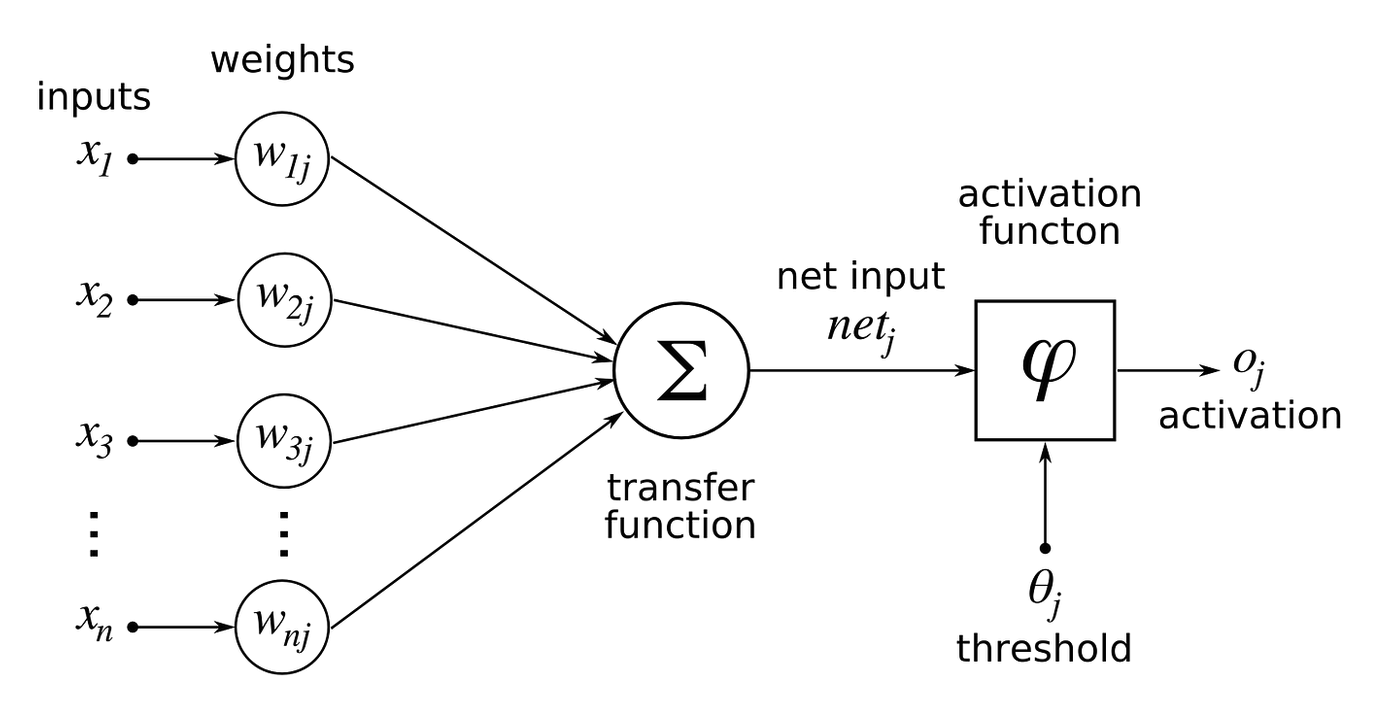
\includegraphics[width=6.3cm,keepaspectratio]{neuron}
\end{center}
\medskip
\begin{examplebox}\footnotesize
The vocabulary is borrowed from biology and the mathematics is not. Nothing below depends on the metaphor, and it is safe to forget it.
\end{examplebox}
\end{column}
\end{columns}
\vspace{1mm}
\src{Feng \& Miao, \emph{AI for Economists}, ch.~9 \S9.1.2.}
\end{frame}

%=============================================================================
\begin{frame}{Why the Nonlinearity Is Not Optional}
\begin{columns}[T]
\begin{column}{0.56\textwidth}
\small
An \textbf{affine} map is a linear map plus a constant --- $\mathbf{W}\mathbf{x}+\mathbf{b}$, which is a layer with its activation stripped off. Suppose we drop $\sigma$ and stack two of them:
\[
  \mathbf{W}_2\bigl(\mathbf{W}_1\mathbf{x}+\mathbf{b}_1\bigr)+\mathbf{b}_2
  =\underbrace{(\mathbf{W}_2\mathbf{W}_1)}_{\text{one matrix}}\mathbf{x}
   +\underbrace{(\mathbf{W}_2\mathbf{b}_1+\mathbf{b}_2)}_{\text{one vector}} .
\]
\medskip

The composition of two affine maps is an affine map. Stack a hundred and it is \emph{still} an affine map --- with a great many parameters and not one extra function it can represent.
\medskip

\textbf{Depth without nonlinearity buys exactly nothing.} The activation is not a detail of implementation; it is the entire reason layers are worth stacking.
\end{column}
\begin{column}{0.41\textwidth}
\begin{takeawaybox}[title=\textbf{Say it as a warning}]\small
If a network is not learning and you have used a linear activation in the hidden layers, you have not built a deep model. You have built a very expensive linear regression.
\end{takeawaybox}
\medskip
\begin{conceptbox}\footnotesize
The same identity read forwards is the useful part: each layer is an \textbf{affine map then a pointwise nonlinearity},
\[
  f=\sigma_L\circ A_L\circ\cdots\circ\sigma_1\circ A_1 ,
\]
with $A_\ell(\mathbf{x})=\mathbf{W}_\ell\mathbf{x}+\mathbf{b}_\ell$.
\end{conceptbox}
\end{column}
\end{columns}
\vspace{1mm}
\src{Feng \& Miao, \emph{AI for Economists}, ch.~9 \S9.1.2.}
\end{frame}

%=============================================================================
\begin{frame}{Layers, and the Object in One Line}
\begin{columns}[T]
\begin{column}{0.50\textwidth}
\small
A \textbf{hidden layer} applies the same construction in parallel,
\[
  \mathbf{h}=\sigma\bigl(\mathbf{W}\mathbf{x}+\mathbf{b}\bigr),
\]
with $\sigma$ applied element by element. Compose $L$ of them and read off the output:
\[
  \mathcal{N}(\mathbf{x};\theta)=\mathbf{W}_{L+1}\,\sigma\bigl(\cdots\sigma(\mathbf{W}_1\mathbf{x}+\mathbf{b}_1)\cdots\bigr)+\mathbf{b}_{L+1}
\]
\medskip

$\theta$ collects every $\mathbf{W}_\ell$ and $\mathbf{b}_\ell$. \textbf{Within a layer, parallel; between layers, in series.}
\end{column}
\begin{column}{0.47\textwidth}
\begin{center}
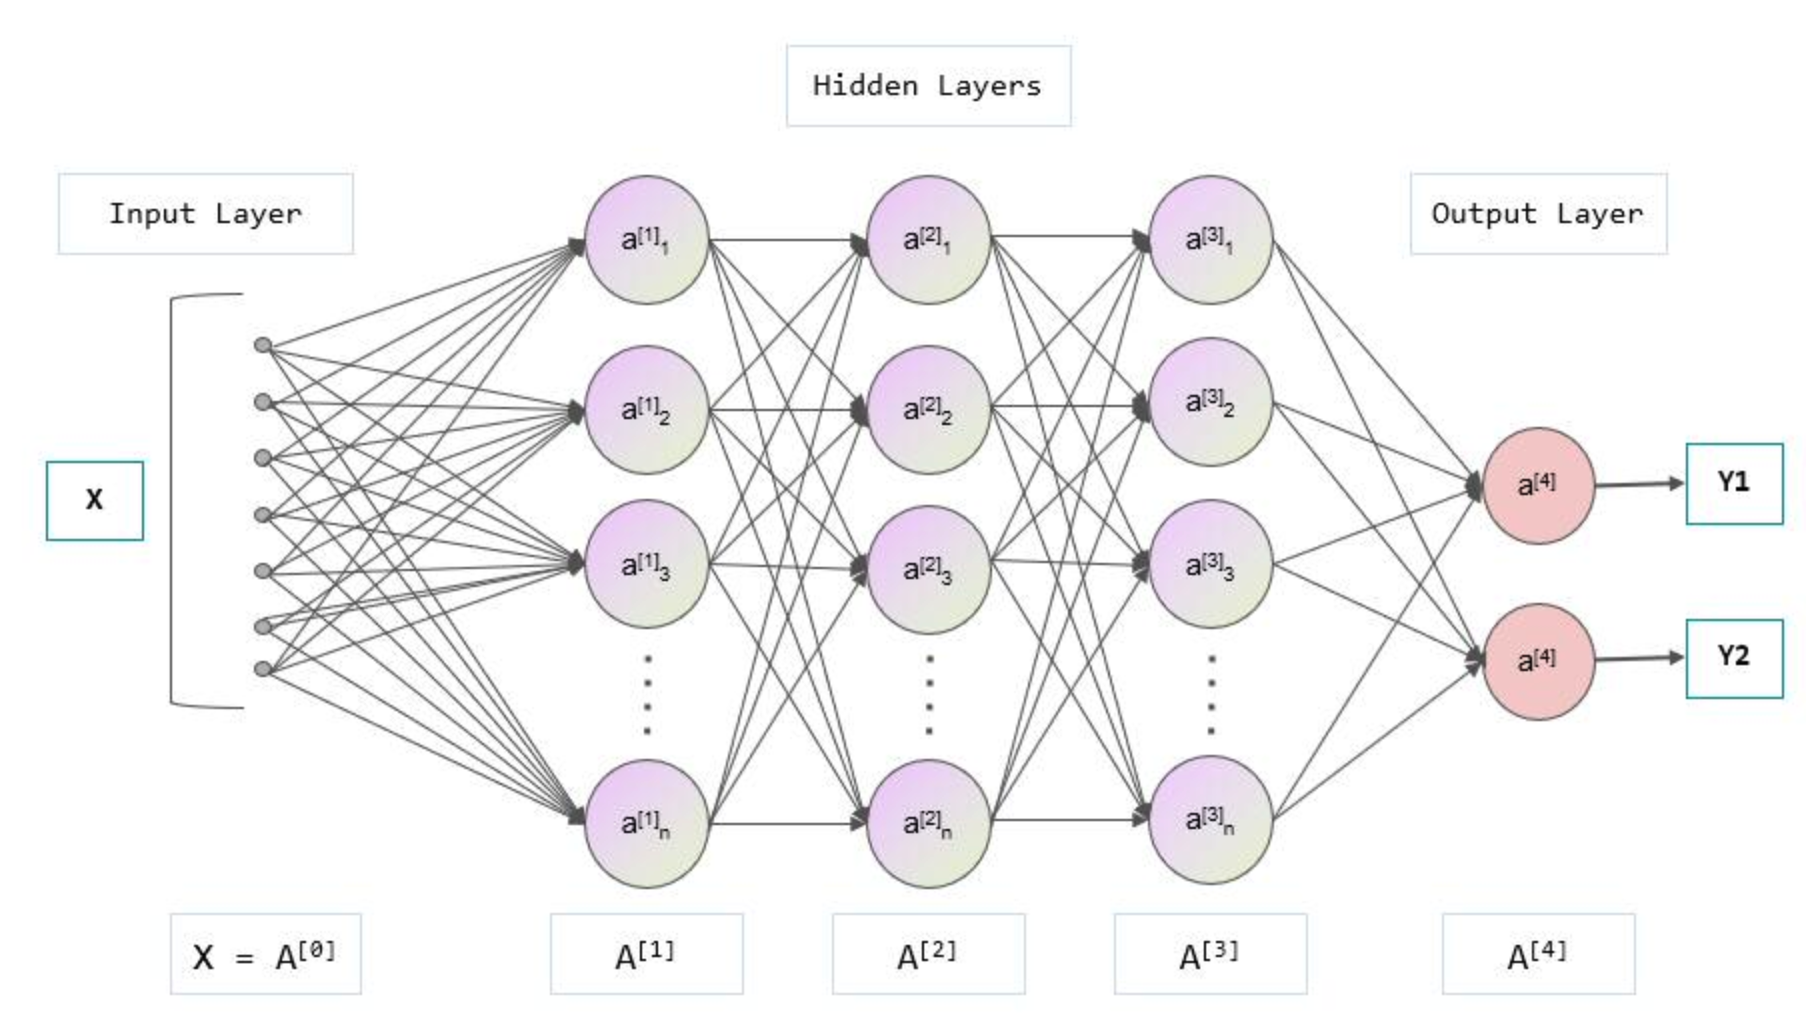
\includegraphics[width=6.6cm,keepaspectratio]{dnn}
\end{center}
\medskip
\begin{takeawaybox}\footnotesize
\textbf{The macro reading:} successive layers are successive transformations of a state into a richer representation --- which is what a dynamic program does to $k_t$ on its way to a decision.
\end{takeawaybox}
\end{column}
\end{columns}
\vspace{1mm}
\src{Feng \& Miao, \emph{AI for Economists}, ch.~9, eq.~(9.8).}
\end{frame}

%=============================================================================
\begin{frame}{XOR: Not Approximated --- Represented}
\begin{columns}[T]
\begin{column}{0.53\textwidth}
\small
The classical objection to a single layer of units is that it cannot represent the exclusive-or. It is true, and one hidden layer settles it \textbf{exactly}. Take
\[
  h_1=\mathrm{ReLU}(x_1+x_2),\quad h_2=\mathrm{ReLU}(x_1+x_2-1),
\]
\[
  \hat y=h_1-2h_2 .
\]
\medskip
\begin{center}\footnotesize
\begin{tabularx}{\linewidth}{@{}>{\centering\arraybackslash}X >{\centering\arraybackslash}X >{\centering\arraybackslash}X >{\centering\arraybackslash}X >{\centering\arraybackslash}X >{\centering\arraybackslash}X@{}}
\toprule
$x_1$ & $x_2$ & $h_1$ & $h_2$ & $\hat y$ & XOR \\
\midrule
$0$ & $0$ & $0$ & $0$ & $0$ & $0$ \\
$0$ & $1$ & $1$ & $0$ & $1$ & $1$ \\
$1$ & $0$ & $1$ & $0$ & $1$ & $1$ \\
$1$ & $1$ & $2$ & $1$ & $0$ & $0$ \\
\bottomrule
\end{tabularx}
\end{center}
\end{column}
\begin{column}{0.44\textwidth}
\begin{takeawaybox}[title=\textbf{Read the last column}]\small
Not ``close to''. \textbf{Equal}, in all four rows, at these exact weights.
\medskip
No linear map in $(x_1,x_2)$ can do this, because the two classes are not linearly separable. \textbf{One hidden layer changes the coordinates until they are.}
\end{takeawaybox}
\medskip
\begin{examplebox}\footnotesize
This is the smallest complete answer to ``what does depth buy?'' --- and it is checkable by hand in thirty seconds, which is why it is here.
\end{examplebox}
\end{column}
\end{columns}
\vspace{1mm}
\src{Goodfellow, Bengio \& Courville (2016) \S6.1; Feng \& Miao, \emph{AI for Economists}, ch.~9 \S9.2.3. Ledger \texttt{xor}: all four rows exact. Code: \repo{tools/figures/s07_generate.py}{s07\_generate.py}, \texttt{run\_xor}.}
\end{frame}

%=============================================================================
\begin{frame}{What Generality Costs, in Parameters}
\begin{columns}[T]
\begin{column}{0.52\textwidth}
\small
A value function in $d=20$ states, and a network of three hidden layers of $256$:
\[
  5{,}376+65{,}792+65{,}792+257=\mathbf{137{,}217}.
\]
Now count the alternatives at the same $d$:

\begin{center}\footnotesize
\begin{tabularx}{\linewidth}{@{}>{\raggedright\arraybackslash}X >{\raggedleft\arraybackslash}p{2.1cm}@{}}
\toprule
\textbf{Object} & \textbf{count} \\
\midrule
the network above & $137{,}217$ \\
\textbf{complete} polynomial, total degree $\le5$ & $53{,}130$ \\
\textbf{tensor-product} polynomial, $5$ per axis & $3.7\times10^{15}$ \\
tensor grid, $5$ points per axis & $9.5\times10^{13}$ \\
\bottomrule
\end{tabularx}
\end{center}
\end{column}
\begin{column}{0.45\textwidth}
\begin{conceptbox}[title=\textbf{Read rows two and three together}]\small
A \textbf{complete} basis keeps every monomial of \emph{total} degree $\le k$ --- $\binom{d+k}{k}$ of them. A \textbf{tensor-product} basis keeps one degree-$k$ factor per axis, $(k+1)^{d}$.
\medskip
Dropping to the complete basis turns $3.7\times10^{15}$ into $53{,}130$ --- \textbf{5.B3's trick}, and the only reason a polynomial is in this table.
\end{conceptbox}
\smallskip
{\footnotesize The network still carries \textbf{two and a half times} the complete basis's coefficients, so be suspicious rather than impressed. \textbf{Parameter count is the wrong axis}; accuracy \emph{per} parameter is, and that is Barron's.}
\end{column}
\end{columns}
\vspace{1mm}
\src{Ledger \texttt{param\_count}. Feng \& Miao, \emph{AI for Economists}, ch.~9 \S9.2.1. Code: \repo{tools/figures/s07_generate.py}{s07\_generate.py}, \texttt{run\_param\_count}.}
\end{frame}

%=============================================================================
\begin{frame}{The Activations You Will Actually Meet}
\begin{center}
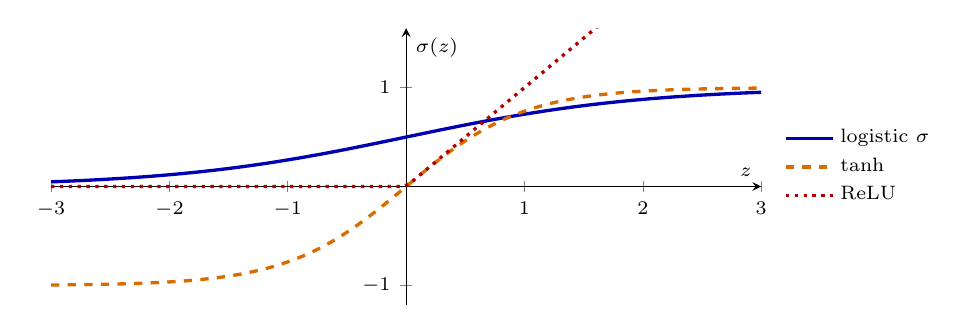
\begin{tikzpicture}
\begin{axis}[
    width=10.6cm, height=5.1cm,
    xmin=-3, xmax=3, ymin=-1.2, ymax=1.6,
    axis lines=middle,
    xlabel={\scriptsize $z$}, ylabel={\scriptsize $\sigma(z)$},
    tick label style={font=\scriptsize}, label style={font=\scriptsize},
    legend style={font=\scriptsize, draw=none, fill=none, at={(1.02,0.5)}, anchor=west},
    legend cell align=left, samples=120]
  \addplot[blue!70!black, very thick, domain=-3:3] {1/(1+exp(-x))};
  \addlegendentry{logistic $\sigma$}
  \addplot[orange!85!black, very thick, dashed, domain=-3:3] {tanh(x)};
  \addlegendentry{$\tanh$}
  \addplot[red!70!black, very thick, dotted, domain=-3:3] {max(0,x)};
  \addlegendentry{ReLU}
\end{axis}
\end{tikzpicture}
\end{center}
\vspace{-1mm}
\begin{columns}[T]
\begin{column}{0.49\textwidth}
\begin{conceptbox}\footnotesize
The logistic and $\tanh$ \textbf{saturate} --- flat in both tails --- and are relatives: $\tanh(z)=2\sigma(2z)-1$. Ranges $(0,1)$ and $(-1,1)$.
\end{conceptbox}
\end{column}
\begin{column}{0.49\textwidth}
\begin{cautionbox}\footnotesize
ReLU is \textbf{piecewise linear}: zero on one side, the identity on the other. It never saturates above, and its derivative is exactly $0$ or $1$.
\end{cautionbox}
\end{column}
\end{columns}
\vspace{1mm}
\src{Ledger \texttt{activations}. Code: \repo{tools/figures/s07_generate.py}{s07\_generate.py}, \texttt{run\_activations}.}
\end{frame}

%=============================================================================
\begin{frame}{The ReLU Family}
\begin{columns}[T]
\begin{column}{0.56\textwidth}
\begin{center}
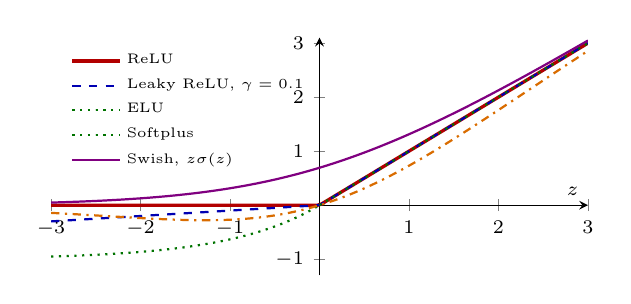
\begin{tikzpicture}
\begin{axis}[
    width=8.4cm, height=4.6cm,
    xmin=-3, xmax=3, ymin=-1.3, ymax=3.1,
    axis lines=middle,
    xlabel={\scriptsize $z$},
    tick label style={font=\scriptsize}, label style={font=\scriptsize},
    legend style={font=\tiny, draw=none, fill=none, at={(0.02,0.98)}, anchor=north west},
    legend cell align=left, samples=140]
  \addplot[red!70!black, very thick, domain=-3:3] {max(0,x)};
  \addlegendentry{ReLU}
  \addplot[blue!70!black, thick, dashed, domain=-3:3] {max(0.1*x,x)};
  \addlegendentry{Leaky ReLU, $\gamma=0.1$}
  \addplot[green!45!black, thick, dotted, domain=-3:0] {exp(x)-1};
  \addplot[green!45!black, thick, dotted, domain=0:3] {x};
  \addlegendentry{ELU}
  \addplot[violet, thick, domain=-3:3] {ln(1+exp(x))};
  \addlegendentry{Softplus}
  \addplot[orange!85!black, thick, dash dot, domain=-3:3] {x/(1+exp(-x))};
  \addlegendentry{Swish, $z\sigma(z)$}
\end{axis}
\end{tikzpicture}
\end{center}
\end{column}
\begin{column}{0.41\textwidth}
\small
Each fixes something about plain ReLU.
\medskip
\begin{itemize}\small\setlength{\itemsep}{1mm}
  \item \textbf{Leaky ReLU} gives the dead side a slope $\gamma$, so a unit that has switched off can come back.
  \item \textbf{ELU} does the same smoothly and saturates at $-1$.
  \item \textbf{Softplus} is ReLU with the corner rounded off --- and is \textbf{differentiable everywhere}, which matters when the model needs a second derivative.
  \item \textbf{Swish} and \textbf{GELU} ($z\Phi(z)$) are the modern defaults in large models; both dip slightly below zero.
\end{itemize}
\end{column}
\end{columns}
\vspace{1mm}
\src{Feng \& Miao, \emph{AI for Economists}, ch.~9 \S9.2.2, Figs.~9.4--9.5. Ledger \texttt{activations}. Code: \repo{tools/figures/s07_generate.py}{s07\_generate.py}.}
\end{frame}

%=============================================================================
\begin{frame}{Saturation, and Where the Vanishing Gradient Begins}
\begin{columns}[T]
\begin{column}{0.54\textwidth}
\small
The logistic derivative is $\sigma'(z)=\sigma(z)(1-\sigma(z))$, whose \textbf{largest possible value is} $\sigma'(0)=0.25$.
\smallskip

7.A3 shows the error signal is multiplied by $\sigma'$ once per layer on the way back --- so with logistic hidden units, by \textbf{at most} $0.25$ each layer:

\begin{center}\footnotesize
\begin{tabularx}{\linewidth}{@{}>{\raggedright\arraybackslash}p{1.9cm} >{\raggedleft\arraybackslash}X >{\raggedleft\arraybackslash}X >{\raggedleft\arraybackslash}X >{\raggedleft\arraybackslash}X@{}}
\toprule
layers $L$ & $1$ & $3$ & $5$ & $7$ \\
\midrule
$0.25^{L}$, at best & $0.25$ & $0.016$ & $\mathbf{0.00098}$ & $6\times10^{-5}$ \\
\bottomrule
\end{tabularx}
\end{center}
{\footnotesize And that is the \emph{best} case; away from $z=0$ it is far worse.}
\end{column}
\begin{column}{0.43\textwidth}
\begin{cautionbox}[title=\textbf{The consequence}]\footnotesize
By five layers the gradient reaching the first layer is a thousandth of the gradient at the last: \textbf{the early layers barely move}, and the network trains as though it were shallow.
\end{cautionbox}
\smallskip
\begin{takeawaybox}\footnotesize
ReLU's derivative is $1$ on the active side --- \textbf{no shrinkage at all}, so the signal survives depth. \textbf{That, not any approximation theorem, is why ReLU is the default for hidden layers.}
\medskip
\textbf{Two qualifications:} a unit off for every sample never returns (hence Leaky ReLU), and the sigmoid keeps the \emph{output}, where a bound is wanted --- 7.B1 uses it.
\end{takeawaybox}
\end{column}
\end{columns}
\vspace{1mm}
\src{Ledger \texttt{activations.chain\_of\_sigmoid\_primes}. Feng \& Miao, \emph{AI for Economists}, ch.~9 \S9.2.2. Code: \repo{tools/figures/s07_generate.py}{s07\_generate.py}.}
\end{frame}

%=============================================================================
\begin{frame}{A Working Guide}
\vspace{-1mm}
\begin{center}\footnotesize
\begin{tabularx}{\linewidth}{@{}>{\raggedright\arraybackslash}p{2.1cm} >{\raggedright\arraybackslash}p{1.9cm} >{\raggedright\arraybackslash}X >{\raggedright\arraybackslash}p{3.5cm}@{}}
\toprule
\textbf{Activation} & \textbf{Range} & \textbf{Main advantage} & \textbf{Typical use} \\
\midrule
ReLU & $[0,\infty)$ & no saturation above; cheap; sparse activation & the default hidden unit \\
Leaky ReLU & $(-\infty,\infty)$ & no dead units & when units are dying \\
ELU & $[-1,\infty)$ & smooth, negative saturation & deeper stacks \\
logistic & $(0,1)$ & reads as a probability & a binary output; \textbf{a bounded policy} \\
$\tanh$ & $(-1,1)$ & zero-centred, smooth & shallow nets; recurrent layers \\
GELU, Swish & $\approx[-0.17,\infty)$ & smooth, often trains better & large models \\
identity & $(-\infty,\infty)$ & none --- and that is the point & \textbf{the output layer of a regression} \\
\bottomrule
\end{tabularx}
\end{center}
\medskip
\begin{columns}[T]
\begin{column}{0.49\textwidth}
\begin{takeawaybox}\footnotesize
\textbf{The row that matters for Block B} is the logistic one, used not as a probability but as a \textbf{bound}: $c=\sigma(\cdot)\times$ cash-on-hand is feasible by construction.
\end{takeawaybox}
\end{column}
\begin{column}{0.49\textwidth}
\begin{cautionbox}\footnotesize
And the last row: putting an activation on the output of a regression silently bounds the prediction. It is a common and expensive mistake.
\end{cautionbox}
\end{column}
\end{columns}
\vspace{1mm}
\src{Feng \& Miao, \emph{AI for Economists}, ch.~9, Table~9.2; the economics column is ours.}
\end{frame}

%=============================================================================
\begin{frame}{An Economist's Reading of the Activation}
\begin{columns}[T]
\begin{column}{0.55\textwidth}
\small
Choosing $\sigma$ is choosing a \textbf{flexible functional form}. You have done it before --- translog, CES, a semi-parametric index --- and the considerations are recognisably the same: how much curvature, where, and at what cost in parameters.
\medskip

There is one difference, and it is the whole difference. A translog is applied \textbf{once}. A network \textbf{composes} its functional form across layers, so what the second layer bends is not the data but the first layer's representation of it.
\end{column}
\begin{column}{0.42\textwidth}
\begin{conceptbox}[title=\textbf{And the classical objection}]\small
``But $\theta$ has no interpretation.'' Correct, and it is not meant to. 7.A1 separated the three jobs: this is \textbf{computation}, and the object being interpreted is the \emph{function}, not the parameters.
\medskip
The policy function is what you report. Nobody reports a Chebyshev coefficient either.
\end{conceptbox}
\end{column}
\end{columns}
\end{frame}

%=============================================================================
\begin{frame}{The Construction: an Approximation Built out of Kinks}
\begin{columns}[T]
\begin{column}{0.55\textwidth}
\small
Take the simplest possible network: one hidden ReLU layer, one input, one output. Written out, it is
\[
  \hat y(x)=a_0+\sum_{i=1}^{N}a_i\,\mathrm{ReLU}(x-b_i).
\]
\medskip

Read the two sets of parameters separately, because they do quite different jobs:
\begin{itemize}\small\setlength{\itemsep}{1.2mm}
  \item the \textbf{shifts} $b_i$ are the \textbf{kink points} --- the places where the marginal slope is allowed to change;
  \item the \textbf{coefficients} $a_i$ \textbf{scale} each piece's contribution, and so set the slope on each interval.
\end{itemize}
\end{column}
\begin{column}{0.42\textwidth}
\begin{takeawaybox}[title=\textbf{You have seen this basis}]\small
Fix the $b_i$ in advance and $\hat y$ is \textbf{linear in the remaining parameters}. It is a regression on a piecewise-linear basis --- 5.B4's elements, with the knots at the $b_i$.
\end{takeawaybox}
\medskip
\begin{examplebox}\footnotesize
Which means the next frame is not a new method. It is 5.B5's \textbf{least squares}, run on a basis you already know.
\end{examplebox}
\end{column}
\end{columns}
\end{frame}

%=============================================================================
\begin{frame}{Worked: $\sin x$ out of Kinks, by Least Squares}
\begin{columns}[T]
\begin{column}{0.56\textwidth}
\begin{center}
\begin{tikzpicture}
\begin{axis}[
    width=8.2cm, height=4.25cm,
    xmin=-3.2, xmax=3.2, ymin=-1.35, ymax=1.35,
    xlabel={\scriptsize $x$},
    tick label style={font=\scriptsize}, label style={font=\scriptsize},
    axis x line*=bottom, axis y line*=left,
    legend style={font=\tiny, draw=none, fill=none, at={(0.5,-0.30)}, anchor=north, legend columns=4}]
  \addplot[very thick, black!45] coordinates {(-3.1416,-0.0000) (-3.1102,-0.0314) (-3.0788,-0.0628) (-3.0473,-0.0941) (-3.0159,-0.1253) (-2.9845,-0.1564) (-2.9531,-0.1874) (-2.9217,-0.2181) (-2.8903,-0.2487) (-2.8588,-0.2790) (-2.8274,-0.3090) (-2.7960,-0.3387) (-2.7646,-0.3681) (-2.7332,-0.3971) (-2.7018,-0.4258) (-2.6704,-0.4540) (-2.6389,-0.4818) (-2.6075,-0.5090) (-2.5761,-0.5358) (-2.5447,-0.5621) (-2.5133,-0.5878) (-2.4819,-0.6129) (-2.4504,-0.6374) (-2.4190,-0.6613) (-2.3876,-0.6845) (-2.3562,-0.7071) (-2.3248,-0.7290) (-2.2934,-0.7501) (-2.2619,-0.7705) (-2.2305,-0.7902) (-2.1991,-0.8090) (-2.1677,-0.8271) (-2.1363,-0.8443) (-2.1049,-0.8607) (-2.0735,-0.8763) (-2.0420,-0.8910) (-2.0106,-0.9048) (-1.9792,-0.9178) (-1.9478,-0.9298) (-1.9164,-0.9409) (-1.8850,-0.9511) (-1.8535,-0.9603) (-1.8221,-0.9686) (-1.7907,-0.9759) (-1.7593,-0.9823) (-1.7279,-0.9877) (-1.6965,-0.9921) (-1.6650,-0.9956) (-1.6336,-0.9980) (-1.6022,-0.9995) (-1.5708,-1.0000) (-1.5394,-0.9995) (-1.5080,-0.9980) (-1.4765,-0.9956) (-1.4451,-0.9921) (-1.4137,-0.9877) (-1.3823,-0.9823) (-1.3509,-0.9759) (-1.3195,-0.9686) (-1.2881,-0.9603) (-1.2566,-0.9511) (-1.2252,-0.9409) (-1.1938,-0.9298) (-1.1624,-0.9178) (-1.1310,-0.9048) (-1.0996,-0.8910) (-1.0681,-0.8763) (-1.0367,-0.8607) (-1.0053,-0.8443) (-0.9739,-0.8271) (-0.9425,-0.8090) (-0.9111,-0.7902) (-0.8796,-0.7705) (-0.8482,-0.7501) (-0.8168,-0.7290) (-0.7854,-0.7071) (-0.7540,-0.6845) (-0.7226,-0.6613) (-0.6912,-0.6374) (-0.6597,-0.6129) (-0.6283,-0.5878) (-0.5969,-0.5621) (-0.5655,-0.5358) (-0.5341,-0.5090) (-0.5027,-0.4818) (-0.4712,-0.4540) (-0.4398,-0.4258) (-0.4084,-0.3971) (-0.3770,-0.3681) (-0.3456,-0.3387) (-0.3142,-0.3090) (-0.2827,-0.2790) (-0.2513,-0.2487) (-0.2199,-0.2181) (-0.1885,-0.1874) (-0.1571,-0.1564) (-0.1257,-0.1253) (-0.0942,-0.0941) (-0.0628,-0.0628) (-0.0314,-0.0314) (0.0000,0.0000) (0.0314,0.0314) (0.0628,0.0628) (0.0942,0.0941) (0.1257,0.1253) (0.1571,0.1564) (0.1885,0.1874) (0.2199,0.2181) (0.2513,0.2487) (0.2827,0.2790) (0.3142,0.3090) (0.3456,0.3387) (0.3770,0.3681) (0.4084,0.3971) (0.4398,0.4258) (0.4712,0.4540) (0.5027,0.4818) (0.5341,0.5090) (0.5655,0.5358) (0.5969,0.5621) (0.6283,0.5878) (0.6597,0.6129) (0.6912,0.6374) (0.7226,0.6613) (0.7540,0.6845) (0.7854,0.7071) (0.8168,0.7290) (0.8482,0.7501) (0.8796,0.7705) (0.9111,0.7902) (0.9425,0.8090) (0.9739,0.8271) (1.0053,0.8443) (1.0367,0.8607) (1.0681,0.8763) (1.0996,0.8910) (1.1310,0.9048) (1.1624,0.9178) (1.1938,0.9298) (1.2252,0.9409) (1.2566,0.9511) (1.2881,0.9603) (1.3195,0.9686) (1.3509,0.9759) (1.3823,0.9823) (1.4137,0.9877) (1.4451,0.9921) (1.4765,0.9956) (1.5080,0.9980) (1.5394,0.9995) (1.5708,1.0000) (1.6022,0.9995) (1.6336,0.9980) (1.6650,0.9956) (1.6965,0.9921) (1.7279,0.9877) (1.7593,0.9823) (1.7907,0.9759) (1.8221,0.9686) (1.8535,0.9603) (1.8850,0.9511) (1.9164,0.9409) (1.9478,0.9298) (1.9792,0.9178) (2.0106,0.9048) (2.0420,0.8910) (2.0735,0.8763) (2.1049,0.8607) (2.1363,0.8443) (2.1677,0.8271) (2.1991,0.8090) (2.2305,0.7902) (2.2619,0.7705) (2.2934,0.7501) (2.3248,0.7290) (2.3562,0.7071) (2.3876,0.6845) (2.4190,0.6613) (2.4504,0.6374) (2.4819,0.6129) (2.5133,0.5878) (2.5447,0.5621) (2.5761,0.5358) (2.6075,0.5090) (2.6389,0.4818) (2.6704,0.4540) (2.7018,0.4258) (2.7332,0.3971) (2.7646,0.3681) (2.7960,0.3387) (2.8274,0.3090) (2.8588,0.2790) (2.8903,0.2487) (2.9217,0.2181) (2.9531,0.1874) (2.9845,0.1564) (3.0159,0.1253) (3.0473,0.0941) (3.0788,0.0628) (3.1102,0.0314) (3.1416,0.0000)};
  \addlegendentry{$\sin x$}
  \addplot[thick, orange!90!black] coordinates {(-3.1416,-0.7779) (-3.1102,-0.7779) (-3.0788,-0.7779) (-3.0473,-0.7779) (-3.0159,-0.7779) (-2.9845,-0.7779) (-2.9531,-0.7779) (-2.9217,-0.7779) (-2.8903,-0.7779) (-2.8588,-0.7779) (-2.8274,-0.7779) (-2.7960,-0.7779) (-2.7646,-0.7779) (-2.7332,-0.7779) (-2.7018,-0.7779) (-2.6704,-0.7779) (-2.6389,-0.7779) (-2.6075,-0.7779) (-2.5761,-0.7779) (-2.5447,-0.7779) (-2.5133,-0.7779) (-2.4819,-0.7779) (-2.4504,-0.7779) (-2.4190,-0.7779) (-2.3876,-0.7779) (-2.3562,-0.7779) (-2.3248,-0.7779) (-2.2934,-0.7779) (-2.2619,-0.7779) (-2.2305,-0.7779) (-2.1991,-0.7779) (-2.1677,-0.7779) (-2.1363,-0.7779) (-2.1049,-0.7779) (-2.0735,-0.7779) (-2.0420,-0.7779) (-2.0106,-0.7779) (-1.9792,-0.7779) (-1.9478,-0.7779) (-1.9164,-0.7779) (-1.8850,-0.7779) (-1.8535,-0.7779) (-1.8221,-0.7779) (-1.7907,-0.7779) (-1.7593,-0.7779) (-1.7279,-0.7779) (-1.6965,-0.7779) (-1.6650,-0.7779) (-1.6336,-0.7779) (-1.6022,-0.7779) (-1.5708,-0.7779) (-1.5394,-0.7779) (-1.5080,-0.7779) (-1.4765,-0.7779) (-1.4451,-0.7779) (-1.4137,-0.7779) (-1.3823,-0.7779) (-1.3509,-0.7779) (-1.3195,-0.7779) (-1.2881,-0.7779) (-1.2566,-0.7779) (-1.2252,-0.7779) (-1.1938,-0.7779) (-1.1624,-0.7779) (-1.1310,-0.7779) (-1.0996,-0.7779) (-1.0681,-0.7779) (-1.0367,-0.7690) (-1.0053,-0.7424) (-0.9739,-0.7158) (-0.9425,-0.6891) (-0.9111,-0.6625) (-0.8796,-0.6358) (-0.8482,-0.6092) (-0.8168,-0.5825) (-0.7854,-0.5559) (-0.7540,-0.5293) (-0.7226,-0.5026) (-0.6912,-0.4760) (-0.6597,-0.4493) (-0.6283,-0.4227) (-0.5969,-0.3961) (-0.5655,-0.3694) (-0.5341,-0.3428) (-0.5027,-0.3161) (-0.4712,-0.2895) (-0.4398,-0.2629) (-0.4084,-0.2362) (-0.3770,-0.2096) (-0.3456,-0.1829) (-0.3142,-0.1563) (-0.2827,-0.1297) (-0.2513,-0.1030) (-0.2199,-0.0764) (-0.1885,-0.0497) (-0.1571,-0.0231) (-0.1257,0.0035) (-0.0942,0.0302) (-0.0628,0.0568) (-0.0314,0.0835) (0.0000,0.1101) (0.0314,0.1368) (0.0628,0.1634) (0.0942,0.1900) (0.1257,0.2167) (0.1571,0.2433) (0.1885,0.2700) (0.2199,0.2966) (0.2513,0.3232) (0.2827,0.3499) (0.3142,0.3765) (0.3456,0.4032) (0.3770,0.4298) (0.4084,0.4564) (0.4398,0.4831) (0.4712,0.5097) (0.5027,0.5364) (0.5341,0.5630) (0.5655,0.5896) (0.5969,0.6163) (0.6283,0.6429) (0.6597,0.6696) (0.6912,0.6962) (0.7226,0.7228) (0.7540,0.7495) (0.7854,0.7761) (0.8168,0.8028) (0.8482,0.8294) (0.8796,0.8561) (0.9111,0.8827) (0.9425,0.9093) (0.9739,0.9360) (1.0053,0.9626) (1.0367,0.9893) (1.0681,0.9915) (1.0996,0.9817) (1.1310,0.9718) (1.1624,0.9619) (1.1938,0.9520) (1.2252,0.9421) (1.2566,0.9322) (1.2881,0.9223) (1.3195,0.9125) (1.3509,0.9026) (1.3823,0.8927) (1.4137,0.8828) (1.4451,0.8729) (1.4765,0.8630) (1.5080,0.8532) (1.5394,0.8433) (1.5708,0.8334) (1.6022,0.8235) (1.6336,0.8136) (1.6650,0.8037) (1.6965,0.7938) (1.7279,0.7840) (1.7593,0.7741) (1.7907,0.7642) (1.8221,0.7543) (1.8535,0.7444) (1.8850,0.7345) (1.9164,0.7246) (1.9478,0.7148) (1.9792,0.7049) (2.0106,0.6950) (2.0420,0.6851) (2.0735,0.6752) (2.1049,0.6653) (2.1363,0.6554) (2.1677,0.6456) (2.1991,0.6357) (2.2305,0.6258) (2.2619,0.6159) (2.2934,0.6060) (2.3248,0.5961) (2.3562,0.5863) (2.3876,0.5764) (2.4190,0.5665) (2.4504,0.5566) (2.4819,0.5467) (2.5133,0.5368) (2.5447,0.5269) (2.5761,0.5171) (2.6075,0.5072) (2.6389,0.4973) (2.6704,0.4874) (2.7018,0.4775) (2.7332,0.4676) (2.7646,0.4577) (2.7960,0.4479) (2.8274,0.4380) (2.8588,0.4281) (2.8903,0.4182) (2.9217,0.4083) (2.9531,0.3984) (2.9845,0.3885) (3.0159,0.3787) (3.0473,0.3688) (3.0788,0.3589) (3.1102,0.3490) (3.1416,0.3391)};
  \addlegendentry{$N=2$}
  \addplot[thick, green!45!black, dashed] coordinates {(-3.1416,-0.6704) (-3.1102,-0.6704) (-3.0788,-0.6704) (-3.0473,-0.6704) (-3.0159,-0.6704) (-2.9845,-0.6704) (-2.9531,-0.6704) (-2.9217,-0.6704) (-2.8903,-0.6704) (-2.8588,-0.6704) (-2.8274,-0.6704) (-2.7960,-0.6704) (-2.7646,-0.6704) (-2.7332,-0.6704) (-2.7018,-0.6704) (-2.6704,-0.6704) (-2.6389,-0.6704) (-2.6075,-0.6704) (-2.5761,-0.6704) (-2.5447,-0.6704) (-2.5133,-0.6704) (-2.4819,-0.6704) (-2.4504,-0.6704) (-2.4190,-0.6704) (-2.3876,-0.6704) (-2.3562,-0.6704) (-2.3248,-0.6704) (-2.2934,-0.6704) (-2.2619,-0.6704) (-2.2305,-0.6704) (-2.1991,-0.6704) (-2.1677,-0.6704) (-2.1363,-0.6704) (-2.1049,-0.6704) (-2.0735,-0.6704) (-2.0420,-0.6704) (-2.0106,-0.6704) (-1.9792,-0.6704) (-1.9478,-0.6704) (-1.9164,-0.6704) (-1.8850,-0.6704) (-1.8535,-0.6731) (-1.8221,-0.6758) (-1.7907,-0.6785) (-1.7593,-0.6813) (-1.7279,-0.6840) (-1.6965,-0.6867) (-1.6650,-0.6894) (-1.6336,-0.6922) (-1.6022,-0.6949) (-1.5708,-0.6976) (-1.5394,-0.7003) (-1.5080,-0.7031) (-1.4765,-0.7058) (-1.4451,-0.7085) (-1.4137,-0.7112) (-1.3823,-0.7139) (-1.3509,-0.7167) (-1.3195,-0.7194) (-1.2881,-0.7221) (-1.2566,-0.7248) (-1.2252,-0.7276) (-1.1938,-0.7303) (-1.1624,-0.7330) (-1.1310,-0.7357) (-1.0996,-0.7384) (-1.0681,-0.7412) (-1.0367,-0.7439) (-1.0053,-0.7466) (-0.9739,-0.7493) (-0.9425,-0.7521) (-0.9111,-0.7548) (-0.8796,-0.7575) (-0.8482,-0.7602) (-0.8168,-0.7630) (-0.7854,-0.7657) (-0.7540,-0.7684) (-0.7226,-0.7711) (-0.6912,-0.7738) (-0.6597,-0.7766) (-0.6283,-0.7793) (-0.5969,-0.7423) (-0.5655,-0.7053) (-0.5341,-0.6683) (-0.5027,-0.6312) (-0.4712,-0.5942) (-0.4398,-0.5572) (-0.4084,-0.5202) (-0.3770,-0.4832) (-0.3456,-0.4462) (-0.3142,-0.4092) (-0.2827,-0.3721) (-0.2513,-0.3351) (-0.2199,-0.2981) (-0.1885,-0.2611) (-0.1571,-0.2241) (-0.1257,-0.1871) (-0.0942,-0.1501) (-0.0628,-0.1131) (-0.0314,-0.0760) (0.0000,-0.0390) (0.0314,-0.0020) (0.0628,0.0350) (0.0942,0.0720) (0.1257,0.1090) (0.1571,0.1460) (0.1885,0.1830) (0.2199,0.2201) (0.2513,0.2571) (0.2827,0.2941) (0.3142,0.3311) (0.3456,0.3681) (0.3770,0.4051) (0.4084,0.4421) (0.4398,0.4791) (0.4712,0.5162) (0.5027,0.5532) (0.5341,0.5902) (0.5655,0.6272) (0.5969,0.6642) (0.6283,0.7012) (0.6597,0.7102) (0.6912,0.7192) (0.7226,0.7282) (0.7540,0.7372) (0.7854,0.7462) (0.8168,0.7552) (0.8482,0.7641) (0.8796,0.7731) (0.9111,0.7821) (0.9425,0.7911) (0.9739,0.8001) (1.0053,0.8091) (1.0367,0.8181) (1.0681,0.8271) (1.0996,0.8360) (1.1310,0.8450) (1.1624,0.8540) (1.1938,0.8630) (1.2252,0.8720) (1.2566,0.8810) (1.2881,0.8900) (1.3195,0.8989) (1.3509,0.9079) (1.3823,0.9169) (1.4137,0.9259) (1.4451,0.9349) (1.4765,0.9439) (1.5080,0.9529) (1.5394,0.9619) (1.5708,0.9708) (1.6022,0.9798) (1.6336,0.9888) (1.6650,0.9978) (1.6965,1.0068) (1.7279,1.0158) (1.7593,1.0248) (1.7907,1.0338) (1.8221,1.0427) (1.8535,1.0517) (1.8850,1.0607) (1.9164,1.0354) (1.9478,1.0102) (1.9792,0.9849) (2.0106,0.9596) (2.0420,0.9343) (2.0735,0.9091) (2.1049,0.8838) (2.1363,0.8585) (2.1677,0.8332) (2.1991,0.8080) (2.2305,0.7827) (2.2619,0.7574) (2.2934,0.7321) (2.3248,0.7069) (2.3562,0.6816) (2.3876,0.6563) (2.4190,0.6310) (2.4504,0.6058) (2.4819,0.5805) (2.5133,0.5552) (2.5447,0.5299) (2.5761,0.5047) (2.6075,0.4794) (2.6389,0.4541) (2.6704,0.4288) (2.7018,0.4036) (2.7332,0.3783) (2.7646,0.3530) (2.7960,0.3277) (2.8274,0.3025) (2.8588,0.2772) (2.8903,0.2519) (2.9217,0.2266) (2.9531,0.2014) (2.9845,0.1761) (3.0159,0.1508) (3.0473,0.1255) (3.0788,0.1003) (3.1102,0.0750) (3.1416,0.0497)};
  \addlegendentry{$N=4$}
  \addplot[thick, RedTitle] coordinates {(-3.1416,-0.4094) (-3.1102,-0.4094) (-3.0788,-0.4094) (-3.0473,-0.4094) (-3.0159,-0.4094) (-2.9845,-0.4094) (-2.9531,-0.4094) (-2.9217,-0.4094) (-2.8903,-0.4094) (-2.8588,-0.4094) (-2.8274,-0.4094) (-2.7960,-0.4094) (-2.7646,-0.4094) (-2.7332,-0.4094) (-2.7018,-0.4094) (-2.6704,-0.4094) (-2.6389,-0.4094) (-2.6075,-0.4094) (-2.5761,-0.4094) (-2.5447,-0.4094) (-2.5133,-0.4094) (-2.4819,-0.4094) (-2.4504,-0.4094) (-2.4190,-0.4334) (-2.3876,-0.4642) (-2.3562,-0.4951) (-2.3248,-0.5259) (-2.2934,-0.5568) (-2.2619,-0.5877) (-2.2305,-0.6185) (-2.1991,-0.6494) (-2.1677,-0.6802) (-2.1363,-0.7111) (-2.1049,-0.7419) (-2.0735,-0.7728) (-2.0420,-0.8036) (-2.0106,-0.8345) (-1.9792,-0.8654) (-1.9478,-0.8962) (-1.9164,-0.9271) (-1.8850,-0.9579) (-1.8535,-0.9888) (-1.8221,-1.0196) (-1.7907,-1.0505) (-1.7593,-1.0814) (-1.7279,-1.0898) (-1.6965,-1.0802) (-1.6650,-1.0707) (-1.6336,-1.0611) (-1.6022,-1.0516) (-1.5708,-1.0421) (-1.5394,-1.0325) (-1.5080,-1.0230) (-1.4765,-1.0135) (-1.4451,-1.0039) (-1.4137,-0.9944) (-1.3823,-0.9848) (-1.3509,-0.9753) (-1.3195,-0.9658) (-1.2881,-0.9562) (-1.2566,-0.9467) (-1.2252,-0.9371) (-1.1938,-0.9276) (-1.1624,-0.9181) (-1.1310,-0.9085) (-1.0996,-0.8990) (-1.0681,-0.8894) (-1.0367,-0.8752) (-1.0053,-0.8518) (-0.9739,-0.8283) (-0.9425,-0.8048) (-0.9111,-0.7813) (-0.8796,-0.7578) (-0.8482,-0.7343) (-0.8168,-0.7108) (-0.7854,-0.6873) (-0.7540,-0.6639) (-0.7226,-0.6404) (-0.6912,-0.6169) (-0.6597,-0.5934) (-0.6283,-0.5699) (-0.5969,-0.5464) (-0.5655,-0.5229) (-0.5341,-0.4995) (-0.5027,-0.4760) (-0.4712,-0.4525) (-0.4398,-0.4290) (-0.4084,-0.4055) (-0.3770,-0.3820) (-0.3456,-0.3575) (-0.3142,-0.3252) (-0.2827,-0.2929) (-0.2513,-0.2605) (-0.2199,-0.2282) (-0.1885,-0.1958) (-0.1571,-0.1635) (-0.1257,-0.1312) (-0.0942,-0.0988) (-0.0628,-0.0665) (-0.0314,-0.0342) (0.0000,-0.0018) (0.0314,0.0305) (0.0628,0.0629) (0.0942,0.0952) (0.1257,0.1275) (0.1571,0.1599) (0.1885,0.1922) (0.2199,0.2246) (0.2513,0.2569) (0.2827,0.2892) (0.3142,0.3216) (0.3456,0.3539) (0.3770,0.3793) (0.4084,0.4037) (0.4398,0.4282) (0.4712,0.4527) (0.5027,0.4771) (0.5341,0.5016) (0.5655,0.5261) (0.5969,0.5505) (0.6283,0.5750) (0.6597,0.5995) (0.6912,0.6239) (0.7226,0.6484) (0.7540,0.6729) (0.7854,0.6973) (0.8168,0.7218) (0.8482,0.7463) (0.8796,0.7708) (0.9111,0.7952) (0.9425,0.8197) (0.9739,0.8442) (1.0053,0.8686) (1.0367,0.8931) (1.0681,0.9050) (1.0996,0.9106) (1.1310,0.9162) (1.1624,0.9218) (1.1938,0.9275) (1.2252,0.9331) (1.2566,0.9387) (1.2881,0.9443) (1.3195,0.9499) (1.3509,0.9555) (1.3823,0.9611) (1.4137,0.9667) (1.4451,0.9724) (1.4765,0.9780) (1.5080,0.9836) (1.5394,0.9892) (1.5708,0.9948) (1.6022,1.0004) (1.6336,1.0060) (1.6650,1.0117) (1.6965,1.0173) (1.7279,1.0229) (1.7593,1.0188) (1.7907,1.0027) (1.8221,0.9866) (1.8535,0.9704) (1.8850,0.9543) (1.9164,0.9382) (1.9478,0.9220) (1.9792,0.9059) (2.0106,0.8898) (2.0420,0.8736) (2.0735,0.8575) (2.1049,0.8413) (2.1363,0.8252) (2.1677,0.8091) (2.1991,0.7929) (2.2305,0.7768) (2.2619,0.7607) (2.2934,0.7445) (2.3248,0.7284) (2.3562,0.7123) (2.3876,0.6961) (2.4190,0.6800) (2.4504,0.6608) (2.4819,0.6311) (2.5133,0.6014) (2.5447,0.5717) (2.5761,0.5419) (2.6075,0.5122) (2.6389,0.4825) (2.6704,0.4527) (2.7018,0.4230) (2.7332,0.3933) (2.7646,0.3636) (2.7960,0.3338) (2.8274,0.3041) (2.8588,0.2744) (2.8903,0.2446) (2.9217,0.2149) (2.9531,0.1852) (2.9845,0.1555) (3.0159,0.1257) (3.0473,0.0960) (3.0788,0.0663) (3.1102,0.0365) (3.1416,0.0068)};
  \addlegendentry{$N=8$}
\end{axis}
\end{tikzpicture}
\end{center}
\end{column}
\begin{column}{0.41\textwidth}
\small
The recipe is entirely familiar:
\begin{enumerate}\small\setlength{\itemsep}{0.6mm}
  \item spread the $b_i$ evenly over $[-\pi,\pi]$;
  \item build a design matrix with columns $\mathrm{ReLU}(x-b_i)$, plus a constant;
  \item get the $a_i$ by \textbf{least squares}.
\end{enumerate}
\medskip
\begin{center}\footnotesize
\begin{tabularx}{\linewidth}{@{}>{\raggedleft\arraybackslash}X >{\raggedleft\arraybackslash}X >{\raggedleft\arraybackslash}X@{}}
\toprule
$N$ & unknowns & $\max|\text{err}|$ \\
\midrule
$2$ & $3$ & $0.7779$ \\
$4$ & $5$ & $0.6704$ \\
$8$ & $9$ & $0.4094$ \\
$16$ & $17$ & $0.2220$ \\
\bottomrule
\end{tabularx}
\end{center}
\end{column}
\end{columns}
\vspace{-2mm}
\begin{takeawaybox}\footnotesize
\textbf{There is no network here yet.} With the shifts fixed this is a linear regression on a piecewise-linear basis --- 5.B5's least squares on 5.B4's elements --- and doubling $N$ roughly halves the error, the $O(h)$ rate of a linear element.
\end{takeawaybox}
\vspace{1mm}
\src{Ledger \texttt{relu\_construction}, \texttt{fig\_relu\_fit\_*}. Code: \repo{tools/figures/s07_generate.py}{s07\_generate.py}, \texttt{run\_relu\_construction}; \repo{labs/L07_ML_and_Deep_Growth.ipynb}{L07} Part 1.}
\end{frame}

%=============================================================================
\begin{frame}{The Turn: Let the Kinks Choose Where to Go}
\begin{columns}[T]
\begin{column}{0.52\textwidth}
\small
Now stop fixing the $b_i$. Train them \textbf{along with} the $a_i$ --- which is exactly what a one-hidden-layer ReLU network is, and nothing more.
\medskip

\begin{center}\footnotesize
\begin{tabularx}{\linewidth}{@{}>{\raggedleft\arraybackslash}p{0.8cm} >{\raggedleft\arraybackslash}X >{\raggedleft\arraybackslash}X >{\raggedleft\arraybackslash}X@{}}
\toprule
$N$ & \textbf{fixed} & \textbf{learned} & \textbf{unknowns} \\
\midrule
$2$ & $0.7779$ & $0.7263$ & $3\to5$ \\
$4$ & $0.6704$ & $0.7235$ & $5\to9$ \\
$8$ & $0.4094$ & $0.0389$ & $9\to17$ \\
$16$ & $0.2220$ & $0.0370$ & $17\to33$ \\
\bottomrule
\end{tabularx}
\end{center}
\medskip
At $N=8$ the error falls from $0.4094$ to $0.0389$ --- \textbf{a factor of ten}, for twice the parameters.
\end{column}
\begin{column}{0.45\textwidth}
\begin{takeawaybox}[title=\textbf{This is the whole session}]\small
\textbf{The basis is no longer chosen in advance.} The approximant decides where the function needs to bend, and puts its kinks there.
\medskip
5.B2 promised exactly this frame: ``let the approximant learn where to bend --- that is what a neural network does''.
\end{takeawaybox}
\medskip
\begin{cautionbox}\footnotesize
\textbf{Read row two honestly.} At $N=4$ the learned version is \emph{worse} ($0.7235$ against $0.6704$). Least squares is solved; training is a non-convex search returning a stationary point. \textbf{The flexibility is not guaranteed.}
\end{cautionbox}
\end{column}
\end{columns}
\vspace{1mm}
\src{Ledger \texttt{relu\_construction.rows}: fixed knots by least squares, learned knots by Adam, 4000 steps. Code: \repo{tools/figures/s07_generate.py}{s07\_generate.py}; \repo{labs/L07_ML_and_Deep_Growth.ipynb}{L07} Part 1.}
\end{frame}

%=============================================================================
\begin{frame}{And on a Function with a Kink in It}
\begin{columns}[T]
\begin{column}{0.46\textwidth}
\begin{center}
\begin{tikzpicture}
\begin{axis}[
    width=6.0cm, height=2.6cm,
    xmin=0, xmax=4, ymin=-0.1, ymax=2.0,
    xlabel={\scriptsize cash on hand $x$}, ylabel={\scriptsize $c(x)$},
    tick label style={font=\scriptsize}, label style={font=\scriptsize},
    axis x line*=bottom, axis y line*=left]
  \addplot[very thick, RedTitle] coordinates {(0.0000,0.0000) (0.0200,0.0200) (0.0400,0.0400) (0.0600,0.0600) (0.0800,0.0800) (0.1000,0.1000) (0.1200,0.1200) (0.1400,0.1400) (0.1600,0.1600) (0.1800,0.1800) (0.2000,0.2000) (0.2200,0.2200) (0.2400,0.2400) (0.2600,0.2600) (0.2800,0.2800) (0.3000,0.3000) (0.3200,0.3200) (0.3400,0.3400) (0.3600,0.3600) (0.3800,0.3800) (0.4000,0.4000) (0.4200,0.4200) (0.4400,0.4400) (0.4600,0.4600) (0.4800,0.4800) (0.5000,0.5000) (0.5200,0.5200) (0.5400,0.5400) (0.5600,0.5600) (0.5800,0.5800) (0.6000,0.6000) (0.6200,0.6200) (0.6400,0.6400) (0.6600,0.6600) (0.6800,0.6800) (0.7000,0.7000) (0.7200,0.7200) (0.7400,0.7400) (0.7600,0.7600) (0.7800,0.7800) (0.8000,0.8000) (0.8200,0.8200) (0.8400,0.8400) (0.8600,0.8600) (0.8800,0.8800) (0.9000,0.9000) (0.9200,0.9200) (0.9400,0.9400) (0.9600,0.9600) (0.9800,0.9800) (1.0000,1.0000) (1.0200,1.0050) (1.0400,1.0100) (1.0600,1.0150) (1.0800,1.0200) (1.1000,1.0250) (1.1200,1.0300) (1.1400,1.0350) (1.1600,1.0400) (1.1800,1.0450) (1.2000,1.0500) (1.2200,1.0550) (1.2400,1.0600) (1.2600,1.0650) (1.2800,1.0700) (1.3000,1.0750) (1.3200,1.0800) (1.3400,1.0850) (1.3600,1.0900) (1.3800,1.0950) (1.4000,1.1000) (1.4200,1.1050) (1.4400,1.1100) (1.4600,1.1150) (1.4800,1.1200) (1.5000,1.1250) (1.5200,1.1300) (1.5400,1.1350) (1.5600,1.1400) (1.5800,1.1450) (1.6000,1.1500) (1.6200,1.1550) (1.6400,1.1600) (1.6600,1.1650) (1.6800,1.1700) (1.7000,1.1750) (1.7200,1.1800) (1.7400,1.1850) (1.7600,1.1900) (1.7800,1.1950) (1.8000,1.2000) (1.8200,1.2050) (1.8400,1.2100) (1.8600,1.2150) (1.8800,1.2200) (1.9000,1.2250) (1.9200,1.2300) (1.9400,1.2350) (1.9600,1.2400) (1.9800,1.2450) (2.0000,1.2500) (2.0200,1.2550) (2.0400,1.2600) (2.0600,1.2650) (2.0800,1.2700) (2.1000,1.2750) (2.1200,1.2800) (2.1400,1.2850) (2.1600,1.2900) (2.1800,1.2950) (2.2000,1.3000) (2.2200,1.3050) (2.2400,1.3100) (2.2600,1.3150) (2.2800,1.3200) (2.3000,1.3250) (2.3200,1.3300) (2.3400,1.3350) (2.3600,1.3400) (2.3800,1.3450) (2.4000,1.3500) (2.4200,1.3550) (2.4400,1.3600) (2.4600,1.3650) (2.4800,1.3700) (2.5000,1.3750) (2.5200,1.3800) (2.5400,1.3850) (2.5600,1.3900) (2.5800,1.3950) (2.6000,1.4000) (2.6200,1.4050) (2.6400,1.4100) (2.6600,1.4150) (2.6800,1.4200) (2.7000,1.4250) (2.7200,1.4300) (2.7400,1.4350) (2.7600,1.4400) (2.7800,1.4450) (2.8000,1.4500) (2.8200,1.4550) (2.8400,1.4600) (2.8600,1.4650) (2.8800,1.4700) (2.9000,1.4750) (2.9200,1.4800) (2.9400,1.4850) (2.9600,1.4900) (2.9800,1.4950) (3.0000,1.5000) (3.0200,1.5050) (3.0400,1.5100) (3.0600,1.5150) (3.0800,1.5200) (3.1000,1.5250) (3.1200,1.5300) (3.1400,1.5350) (3.1600,1.5400) (3.1800,1.5450) (3.2000,1.5500) (3.2200,1.5550) (3.2400,1.5600) (3.2600,1.5650) (3.2800,1.5700) (3.3000,1.5750) (3.3200,1.5800) (3.3400,1.5850) (3.3600,1.5900) (3.3800,1.5950) (3.4000,1.6000) (3.4200,1.6050) (3.4400,1.6100) (3.4600,1.6150) (3.4800,1.6200) (3.5000,1.6250) (3.5200,1.6300) (3.5400,1.6350) (3.5600,1.6400) (3.5800,1.6450) (3.6000,1.6500) (3.6200,1.6550) (3.6400,1.6600) (3.6600,1.6650) (3.6800,1.6700) (3.7000,1.6750) (3.7200,1.6800) (3.7400,1.6850) (3.7600,1.6900) (3.7800,1.6950) (3.8000,1.7000) (3.8200,1.7050) (3.8400,1.7100) (3.8600,1.7150) (3.8800,1.7200) (3.9000,1.7250) (3.9200,1.7300) (3.9400,1.7350) (3.9600,1.7400) (3.9800,1.7450) (4.0000,1.7500)};
  \draw[gray!70, dashed] (axis cs:1,-0.1) -- (axis cs:1,1.3);
  \node[font=\tiny, anchor=west, gray!50!black] at (axis cs:1.05,0.45) {the constraint binds};
\end{axis}
\end{tikzpicture}
\end{center}
{\footnotesize \textbf{Same construction, new target:} $c(x)=\min\{x,\,1+0.25(x-1)\}$ --- below the limit the household consumes everything, above it a fraction. \textbf{2.A1's kink}, at $x=1$.}
\medskip

{\footnotesize \textbf{Why the fixed version fails.} Spread evenly, the two knots land at $x=1.33$ and $2.67$, so a straight segment has to bend across the corner. And no $N$ rescues it: evenly spaced knots almost never land on a kink.}
\end{column}
\begin{column}{0.51\textwidth}
\begin{center}\footnotesize
\begin{tabularx}{\linewidth}{@{}>{\raggedleft\arraybackslash}p{0.5cm} >{\raggedleft\arraybackslash}X >{\raggedleft\arraybackslash}X >{\raggedleft\arraybackslash}p{1.7cm}@{}}
\toprule
 & \multicolumn{2}{c}{$\max|\text{err}|$, knots} & \textbf{learned knot} \\
$N$ & \textbf{fixed} & \textbf{learned} & \textbf{nearest $x=1$} \\
\midrule
$2$ & $0.7339$ & $\mathbf{0.0027}$ & $1.0000$ \\
$4$ & $0.5090$ & $\mathbf{0.0050}$ & $1.0000$ \\
$8$ & $0.2678$ & $\mathbf{0.0065}$ & $1.0017$ \\
\bottomrule
\end{tabularx}
\end{center}
\smallskip
\begin{takeawaybox}\footnotesize
\textbf{Look at the last column.} With two kinks to spend, training puts one at $1.0000$ --- \textbf{the true kink, to four decimals}. Nobody told it where the constraint binds, and the error falls \textbf{$274\times$}.
\end{takeawaybox}
\end{column}
\end{columns}
\vspace{1mm}
\src{Ledger \texttt{relu\_construction.kinked\_rows}; code \repo{tools/figures/s07_generate.py}{s07\_generate.py}, \repo{labs/L07_ML_and_Deep_Growth.ipynb}{L07} Part 1. 5.B4 solved this by \emph{putting a boundary at the kink} --- which requires knowing where it is.}
\end{frame}

%=============================================================================
\begin{frame}{Universal Approximation: What You Just Built}
\begin{columns}[T]
\begin{column}{0.54\textwidth}
\begin{conceptbox}[title=\textbf{Universal approximation}]\small
Any continuous function on $[0,1]^{d}$ can be approximated \textbf{uniformly}, to any accuracy, by a network with a \emph{single} hidden layer:
\[
  \hat f(\mathbf{x})=\sum_{j=1}^{m}v_j\,\sigma\bigl(\mathbf{w}_j^{\top}\mathbf{x}+b_j\bigr)+c .
\]
Cybenko (1989) for sigmoidal $\sigma$; Hornik, Stinchcombe \& White (1989) more generally.
\end{conceptbox}
\smallskip
\small
The previous three frames \emph{were} the construction: a weighted sum of shifted kinks bends to fit any curve. \textbf{One hidden unit is one building block; adding units shrinks the error.}
\end{column}
\begin{column}{0.43\textwidth}
\begin{takeawaybox}\small
The nonlinearity is the glue: take $\sigma$ away and the sum collapses to one straight line.
\end{takeawaybox}
\medskip
\begin{examplebox}\footnotesize
\textbf{Do not be too impressed.} Polynomials are dense in the continuous functions on a compact set too --- Stone--Weierstrass, 5.B2's opening. Universality is not what distinguishes a network. \textbf{The rate is.}
\end{examplebox}
\end{column}
\end{columns}
\vspace{1mm}
\src{Cybenko (1989); Hornik, Stinchcombe \& White (1989). Feng \& Miao, \emph{AI for Economists}, ch.~9, Thm.~9.1.}
\end{frame}

%=============================================================================
\begin{frame}{Four Things the Theorem Does Not Say}
\begin{columns}[T]
\begin{column}{0.53\textwidth}
\small
\begin{enumerate}\small\setlength{\itemsep}{1.4mm}
  \item \textbf{Not how many units.} ``There exists $m$'' --- and $m$ may be astronomically large. The theorem is silent on efficiency.
  \item \textbf{Not how to find it.} It asserts that good weights \emph{exist}. Finding them is the non-convex search of 7.A3, which promises only a stationary point.
  \item \textbf{Not how much data.} Approximating a known function is not estimating an unknown one from a finite sample.
  \item \textbf{Not that it will generalise.} Fitting the sample and fitting the function are different achievements.
\end{enumerate}
\end{column}
\begin{column}{0.44\textwidth}
\begin{cautionbox}[title=\textbf{Keep these apart}]\small
\textbf{Approximation} $\neq$ \textbf{optimization} $\neq$ \textbf{generalization}.
\medskip
Universal approximation speaks to the first only. 7.A3 is the second. The validation discipline of 7.B3 is the third.
\end{cautionbox}
\medskip
\begin{examplebox}\footnotesize
The $N=4$ row two frames ago is (2) in miniature: the better approximation existed --- the fixed-knot fit found it --- and training did not.
\end{examplebox}
\end{column}
\end{columns}
\vspace{1mm}
\src{Feng \& Miao, \emph{AI for Economists}, ch.~9 \S9.1.4. \textbf{Which $\sigma$ work?} Leshno, Lin, Pinkus \& Schocken (1993): a network is universal \emph{if and only if} $\sigma$ is not a polynomial --- so the requirement is remarkably weak, and a polynomial activation is exactly the case that fails.}
\end{frame}

%=============================================================================
\begin{frame}{Barron's Theorem: a Rate That Does Not See $d$}
\begin{columns}[T]
\begin{column}{0.55\textwidth}
\footnotesize
\textbf{In words.} Double the hidden units and the squared error halves --- and \textbf{that rate does not deteriorate as the number of state variables grows}, provided $f$ is in the Barron class.
\smallskip
\begin{conceptbox}[title=\textbf{Barron (1993), Proposition 1}]\footnotesize
With $m$ hidden units, on a ball $B_r$ and averaging against $\mu$,
\[
  \int_{B_r}\bigl(f-\hat f_m\bigr)^{2}\mathrm{d}\mu\;\le\;\frac{(2rC_f)^{2}}{m},
  \qquad C_f=\!\int\!\lVert\boldsymbol\omega\rVert\,|\hat f(\boldsymbol\omega)|\,\mathrm{d}\boldsymbol\omega .
\]
$C_f$ is $f$'s total \textbf{wiggliness}, weighted by frequency; the \textbf{Barron class} is the functions whose Fourier mass sits at low frequencies.
\end{conceptbox}
\smallskip
\small
The bound is $O(1/m)$ with $d$ \textbf{absent from it}. A fixed series basis manages only $O(m^{-2/d})$.
\end{column}
\begin{column}{0.42\textwidth}
\begin{takeawaybox}[title=\textbf{Why the difference}]\small
\textbf{A grid basis is fixed}: resolution $k$ per axis needs $k^{d}$ pieces, most of them parked where $f$ barely moves. That is the curse.
\medskip
\textbf{A neuron is a ridge} $\sigma(\mathbf{w}^{\top}\mathbf{x}+b)$ --- a soft step along a \emph{learned} direction $\mathbf{w}$. The network spends its $m$ units where $f$ actually varies.
\end{takeawaybox}
\medskip
{\footnotesize That is the mechanism you watched find the kink at $1.0000$, now stated as a theorem.}
\end{column}
\end{columns}
\vspace{1mm}
\src{Barron (1993), \emph{IEEE Trans.\ Inf.\ Theory}, Prop.~1; Feng \& Miao, \emph{AI for Economists}, ch.~9, Thm.~9.2.}
\end{frame}

%=============================================================================
\begin{frame}{Where the Dimension Actually Went}
\begin{columns}[T]
\begin{column}{0.55\textwidth}
\small
It is tempting to read $O(1/m)$ as ``neural networks defeat the curse of dimensionality''. \textbf{That reading does not survive contact with the constant.}
\medskip

$C_f=\int\lVert\boldsymbol\omega\rVert\,|\hat f(\boldsymbol\omega)|\,\mathrm{d}\boldsymbol\omega$ is itself an integral over $\mathbb{R}^{d}$. For many ordinary functions it grows with $d$; for many others it is infinite, which puts them outside the class.
\medskip

\textbf{The dimension did not disappear. It moved house} --- into the constant, and into the narrowness of the class.
\end{column}
\begin{column}{0.42\textwidth}
\begin{cautionbox}[title=\textbf{What is genuinely true}]\small
Where $C_f$ stays moderate as $d$ grows, a network's accuracy per parameter degrades far more gracefully than a tensor basis. \textbf{That is real and useful} --- and it is not the statement ``the curse is beaten''.
\medskip
So: a network is right when $d$ is large \emph{and} a few ridge directions express the function. \textbf{Whether that holds for your model is empirical}, which is why 7.B3 measures.
\end{cautionbox}
\end{column}
\end{columns}
\vspace{1mm}
\src{Feng \& Miao, \emph{AI for Economists}, ch.~9 \S9.1.5. Barron (1994), \emph{Machine Learning}, Thm.~3 adds the estimation side: risk $O(C_f^{2}/m)+O((md/n)\log n)$, optimised at $m\asymp C_f\sqrt{n/(d\log n)}$.}
\end{frame}

%=============================================================================
\begin{frame}{The Sharper Result: What a Fixed Basis Cannot Do}
\begin{columns}[T]
\begin{column}{0.54\textwidth}
\small
Barron's \textbf{Theorem 6} is the one that does the real work, and it is a \emph{lower} bound. On the same Barron class, \textbf{any} approximation built from a basis chosen \emph{in advance} --- polynomials, splines, wavelets, Chebyshev, any of them --- cannot do better than
\[
  O\bigl(m^{-2/d}\bigr).
\]
\medskip

Read that against the network's $O(1/m)$. The gap is not between polynomials and networks as such. \textbf{It is between a basis fixed before you look at $f$ and a basis adapted to $f$.}
\end{column}
\begin{column}{0.43\textwidth}
\begin{takeawaybox}[title=\textbf{The through-line of this course}]\small
5.B2 chose a basis. 5.B3 chose a better one. 5.B4 chose where to break it.
\medskip
Every one of those choices was made \textbf{before} the solution was known --- and Theorem 6 says that is precisely what caps the rate.
\end{takeawaybox}
\medskip
\begin{examplebox}\footnotesize
So the theorem names the thing to give up. It does not promise that giving it up will go well, and the next frames measure a case where it does not.
\end{examplebox}
\end{column}
\end{columns}
\vspace{1mm}
\src{Barron (1993), Thm.~6, p.~942; Feng \& Miao, \emph{AI for Economists}, ch.~9 \S9.1.5.}
\end{frame}

%=============================================================================
\begin{frame}{The Rates, Side by Side}
\vspace{-1mm}
\begin{center}\footnotesize
\begin{tabularx}{\linewidth}{@{}>{\raggedright\arraybackslash}p{2.3cm} >{\raggedright\arraybackslash}p{3.0cm} >{\raggedright\arraybackslash}X >{\raggedright\arraybackslash}p{2.6cm}@{}}
\toprule
\textbf{Function class} & \textbf{Approximator} & \textbf{Size needed for accuracy $\varepsilon$} & \textbf{Source} \\
\midrule
$k$-times smooth & tensor-grid polynomial & $\varepsilon^{-d/k}$ & Mhaskar (1996) \\
$k$-times smooth & \emph{any} $m$-parameter continuous method & no better than $m^{-k/d}$ & DeVore, Howard \& Micchelli (1989) \\
Barron class & any \textbf{fixed} basis & no better than $m^{-2/d}$ & Barron (1993), Thm.~6 \\
Barron class & one hidden layer & $m\ge(2rC_f/\varepsilon)^{2}$ --- \textbf{no $d$ in the exponent} & Barron (1993), Prop.~1 \\
compositional (binary tree) & a matching deep network & $O\bigl((d-1)\varepsilon^{-2/k}\bigr)$ vs.\ shallow $O(\varepsilon^{-d/k})$ & Poggio et al.\ (2017) \\
\bottomrule
\end{tabularx}
\end{center}
\medskip
\begin{columns}[T]
\begin{column}{0.49\textwidth}
\begin{takeawaybox}\footnotesize
\textbf{Rows one and two are Session 5's world}, and row two is the discouraging one: the $m^{-k/d}$ ceiling binds on \emph{any} method with a fixed parameterisation, not just on the ones we tried.
\end{takeawaybox}
\end{column}
\begin{column}{0.49\textwidth}
\begin{cautionbox}\footnotesize
\textbf{Rows three to five buy their escape with an assumption} --- membership of the Barron class, or a compositional structure. Neither is free, and neither is checkable for a value function you have not solved for.
\end{cautionbox}
\end{column}
\end{columns}
\vspace{1mm}
\src{Feng \& Miao, \emph{AI for Economists}, ch.~9, Table~9.1.}
\end{frame}

%=============================================================================
\begin{frame}{Depth: the Other Axis}
\begin{columns}[T]
\begin{column}{0.54\textwidth}
\small
Everything so far has bought accuracy with \textbf{width} --- more units in one layer. Depth is a different purchase, and for some functions a far better one.
\medskip

Consider a function built as a \textbf{binary tree of two-variable compositions} --- $f$ is a function of pairs, of pairs, of pairs. A shallow network needs $O(\varepsilon^{-d/k})$ units; a deep network \textbf{whose architecture matches the tree} needs $O\bigl((d-1)\varepsilon^{-2/k}\bigr)$.
\medskip

The exponent stops depending on $d$. \textbf{But only if the function really has that structure} and the network is shaped like it.
\end{column}
\begin{column}{0.43\textwidth}
\begin{conceptbox}[title=\textbf{Theorem (Eldan \& Shamir 2016)}]\small
There is a function on $\mathbb{R}^{d}$ that a \textbf{three-layer} network represents with $O(d^{19/4})$ units, and that \textbf{no two-layer} network can approximate with fewer than $e^{cd}$ units.
\medskip
Polynomial against exponential. \textbf{Depth is not a matter of taste.}
\end{conceptbox}
\medskip
\begin{examplebox}\footnotesize
Compare 7.A4's message: \emph{architecture is an assumption about the target}. This is the same statement, proved.
\end{examplebox}
\end{column}
\end{columns}
\vspace{1mm}
\src{Mhaskar (1996); DeVore, Howard \& Micchelli (1989); Poggio, Mhaskar, Rosasco, Miranda \& Liao (2017); Eldan \& Shamir (2016), Thm.~1. Feng \& Miao, \emph{AI for Economists}, ch.~9 \S9.1.6.}
\end{frame}

%=============================================================================
\begin{frame}{Why Composition Is Economically Natural}
\begin{columns}[T]
\begin{column}{0.53\textwidth}
\small
The compositional assumption is not an exotic one to make about an economic model. Two familiar cases:
\medskip

\textbf{A decision.} Raw data $\to$ a small number of cognitive variables, beliefs and expectations $\to$ a choice. Three layers, and the middle one is genuinely low-dimensional --- which is what the whole recursive-methods apparatus assumes when it writes down a state.
\medskip

\textbf{Aggregation.} Individual decisions $\to$ group or sectoral outcomes $\to$ aggregates. Micro to macro \emph{is} a composition, and the intermediate objects are the ones we name.
\end{column}
\begin{column}{0.44\textwidth}
\begin{takeawaybox}[title=\textbf{The connection worth making}]\small
Krusell--Smith asserts that the aggregate law of motion depends on $\Gamma$ only through its \textbf{mean}. That is a compositional hypothesis --- a one-dimensional bottleneck asserted by the modeller.
\medskip
S8's DeepHAM keeps the structure and \textbf{learns the bottleneck} instead of asserting it.
\end{takeawaybox}
\medskip
\begin{examplebox}\footnotesize
7.A1's manifold hypothesis, met a third time: the same idea in pixels, in states, and now in a theorem about depth.
\end{examplebox}
\end{column}
\end{columns}
\vspace{1mm}
\src{Feng \& Miao, \emph{AI for Economists}, ch.~9 \S9.1.6.}
\end{frame}

%=============================================================================
\begin{frame}{Measured: a Network Against Chebyshev}
\vspace{-1mm}
\begin{columns}[T]
\begin{column}{0.49\textwidth}
\begin{center}
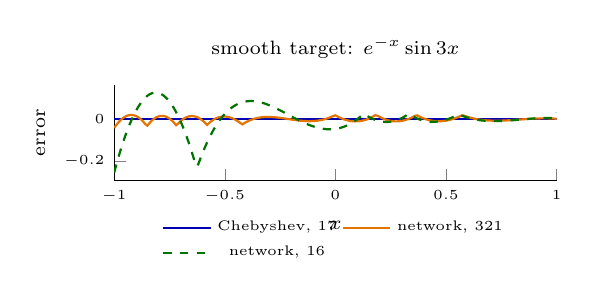
\begin{tikzpicture}
\begin{axis}[
    width=7.2cm, height=2.8cm,
    title={\scriptsize smooth target: $e^{-x}\sin 3x$},
    xmin=-1, xmax=1, xlabel={\scriptsize $x$},
    ylabel={\scriptsize error},
    tick label style={font=\tiny}, label style={font=\tiny}, title style={font=\scriptsize},
    axis x line*=bottom, axis y line*=left,
    legend style={font=\tiny, draw=none, fill=none, at={(0.5,-0.30)}, anchor=north, legend columns=2}]
  \addplot[thick, blue!70!black] coordinates {(-1.0000,0.0000) (-0.9900,-0.0000) (-0.9800,-0.0000) (-0.9700,-0.0000) (-0.9600,-0.0000) (-0.9500,0.0000) (-0.9400,0.0000) (-0.9300,0.0000) (-0.9200,0.0000) (-0.9100,0.0000) (-0.9000,0.0000) (-0.8900,0.0000) (-0.8800,0.0000) (-0.8700,-0.0000) (-0.8600,-0.0000) (-0.8500,-0.0000) (-0.8400,-0.0000) (-0.8300,-0.0000) (-0.8200,-0.0000) (-0.8100,-0.0000) (-0.8000,-0.0000) (-0.7900,-0.0000) (-0.7800,0.0000) (-0.7700,0.0000) (-0.7600,0.0000) (-0.7500,0.0000) (-0.7400,0.0000) (-0.7300,0.0000) (-0.7200,0.0000) (-0.7100,0.0000) (-0.7000,0.0000) (-0.6900,0.0000) (-0.6800,0.0000) (-0.6700,0.0000) (-0.6600,0.0000) (-0.6500,-0.0000) (-0.6400,-0.0000) (-0.6300,-0.0000) (-0.6200,-0.0000) (-0.6100,-0.0000) (-0.6000,-0.0000) (-0.5900,-0.0000) (-0.5800,-0.0000) (-0.5700,-0.0000) (-0.5600,-0.0000) (-0.5500,-0.0000) (-0.5400,-0.0000) (-0.5300,-0.0000) (-0.5200,-0.0000) (-0.5100,-0.0000) (-0.5000,0.0000) (-0.4900,0.0000) (-0.4800,0.0000) (-0.4700,0.0000) (-0.4600,0.0000) (-0.4500,0.0000) (-0.4400,0.0000) (-0.4300,0.0000) (-0.4200,0.0000) (-0.4100,0.0000) (-0.4000,0.0000) (-0.3900,0.0000) (-0.3800,0.0000) (-0.3700,0.0000) (-0.3600,0.0000) (-0.3500,0.0000) (-0.3400,-0.0000) (-0.3300,-0.0000) (-0.3200,-0.0000) (-0.3100,-0.0000) (-0.3000,-0.0000) (-0.2900,-0.0000) (-0.2800,-0.0000) (-0.2700,-0.0000) (-0.2600,-0.0000) (-0.2500,-0.0000) (-0.2400,-0.0000) (-0.2300,-0.0000) (-0.2200,-0.0000) (-0.2100,-0.0000) (-0.2000,-0.0000) (-0.1900,-0.0000) (-0.1800,-0.0000) (-0.1700,0.0000) (-0.1600,0.0000) (-0.1500,0.0000) (-0.1400,0.0000) (-0.1300,0.0000) (-0.1200,0.0000) (-0.1100,0.0000) (-0.1000,0.0000) (-0.0900,0.0000) (-0.0800,0.0000) (-0.0700,0.0000) (-0.0600,0.0000) (-0.0500,0.0000) (-0.0400,0.0000) (-0.0300,0.0000) (-0.0200,0.0000) (-0.0100,0.0000) (0.0000,0.0000) (0.0100,-0.0000) (0.0200,-0.0000) (0.0300,-0.0000) (0.0400,-0.0000) (0.0500,-0.0000) (0.0600,-0.0000) (0.0700,-0.0000) (0.0800,-0.0000) (0.0900,-0.0000) (0.1000,-0.0000) (0.1100,-0.0000) (0.1200,-0.0000) (0.1300,-0.0000) (0.1400,-0.0000) (0.1500,-0.0000) (0.1600,-0.0000) (0.1700,-0.0000) (0.1800,-0.0000) (0.1900,0.0000) (0.2000,0.0000) (0.2100,0.0000) (0.2200,0.0000) (0.2300,0.0000) (0.2400,0.0000) (0.2500,0.0000) (0.2600,0.0000) (0.2700,0.0000) (0.2800,0.0000) (0.2900,0.0000) (0.3000,0.0000) (0.3100,0.0000) (0.3200,0.0000) (0.3300,0.0000) (0.3400,0.0000) (0.3500,0.0000) (0.3600,-0.0000) (0.3700,-0.0000) (0.3800,-0.0000) (0.3900,-0.0000) (0.4000,-0.0000) (0.4100,-0.0000) (0.4200,-0.0000) (0.4300,-0.0000) (0.4400,-0.0000) (0.4500,-0.0000) (0.4600,-0.0000) (0.4700,-0.0000) (0.4800,-0.0000) (0.4900,-0.0000) (0.5000,-0.0000) (0.5100,-0.0000) (0.5200,0.0000) (0.5300,0.0000) (0.5400,0.0000) (0.5500,0.0000) (0.5600,0.0000) (0.5700,0.0000) (0.5800,0.0000) (0.5900,0.0000) (0.6000,0.0000) (0.6100,0.0000) (0.6200,0.0000) (0.6300,0.0000) (0.6400,0.0000) (0.6500,0.0000) (0.6600,0.0000) (0.6700,-0.0000) (0.6800,-0.0000) (0.6900,-0.0000) (0.7000,-0.0000) (0.7100,-0.0000) (0.7200,-0.0000) (0.7300,-0.0000) (0.7400,-0.0000) (0.7500,-0.0000) (0.7600,-0.0000) (0.7700,-0.0000) (0.7800,-0.0000) (0.7900,0.0000) (0.8000,0.0000) (0.8100,0.0000) (0.8200,0.0000) (0.8300,0.0000) (0.8400,0.0000) (0.8500,0.0000) (0.8600,0.0000) (0.8700,0.0000) (0.8800,0.0000) (0.8900,-0.0000) (0.9000,-0.0000) (0.9100,-0.0000) (0.9200,-0.0000) (0.9300,-0.0000) (0.9400,-0.0000) (0.9500,-0.0000) (0.9600,0.0000) (0.9700,0.0000) (0.9800,0.0000) (0.9900,0.0000) (1.0000,-0.0000)};
  \addlegendentry{Chebyshev, 17}
  \addplot[thick, orange!90!black] coordinates {(-1.0000,-0.0416) (-0.9900,-0.0268) (-0.9800,-0.0140) (-0.9700,-0.0031) (-0.9600,0.0057) (-0.9500,0.0124) (-0.9400,0.0171) (-0.9300,0.0197) (-0.9200,0.0201) (-0.9100,0.0184) (-0.9000,0.0145) (-0.8900,0.0085) (-0.8800,0.0003) (-0.8700,-0.0101) (-0.8600,-0.0228) (-0.8500,-0.0309) (-0.8400,-0.0177) (-0.8300,-0.0066) (-0.8200,0.0022) (-0.8100,0.0089) (-0.8000,0.0133) (-0.7900,0.0156) (-0.7800,0.0157) (-0.7700,0.0136) (-0.7600,0.0094) (-0.7500,0.0030) (-0.7400,-0.0054) (-0.7300,-0.0160) (-0.7200,-0.0286) (-0.7100,-0.0202) (-0.7000,-0.0094) (-0.6900,-0.0006) (-0.6800,0.0062) (-0.6700,0.0110) (-0.6600,0.0140) (-0.6500,0.0150) (-0.6400,0.0142) (-0.6300,0.0116) (-0.6200,0.0073) (-0.6100,0.0011) (-0.6000,-0.0067) (-0.5900,-0.0162) (-0.5800,-0.0273) (-0.5700,-0.0173) (-0.5600,-0.0087) (-0.5500,-0.0016) (-0.5400,0.0041) (-0.5300,0.0083) (-0.5200,0.0111) (-0.5100,0.0126) (-0.5000,0.0129) (-0.4900,0.0118) (-0.4800,0.0096) (-0.4700,0.0062) (-0.4600,0.0017) (-0.4500,-0.0039) (-0.4400,-0.0104) (-0.4300,-0.0180) (-0.4200,-0.0244) (-0.4100,-0.0177) (-0.4000,-0.0119) (-0.3900,-0.0068) (-0.3800,-0.0025) (-0.3700,0.0011) (-0.3600,0.0041) (-0.3500,0.0065) (-0.3400,0.0083) (-0.3300,0.0095) (-0.3200,0.0104) (-0.3100,0.0107) (-0.3000,0.0107) (-0.2900,0.0104) (-0.2800,0.0097) (-0.2700,0.0088) (-0.2600,0.0077) (-0.2500,0.0064) (-0.2400,0.0050) (-0.2300,0.0035) (-0.2200,0.0019) (-0.2100,0.0003) (-0.2000,-0.0013) (-0.1900,-0.0029) (-0.1800,-0.0043) (-0.1700,-0.0056) (-0.1600,-0.0068) (-0.1500,-0.0078) (-0.1400,-0.0085) (-0.1300,-0.0090) (-0.1200,-0.0093) (-0.1100,-0.0092) (-0.1000,-0.0087) (-0.0900,-0.0079) (-0.0800,-0.0067) (-0.0700,-0.0050) (-0.0600,-0.0029) (-0.0500,-0.0004) (-0.0400,0.0027) (-0.0300,0.0063) (-0.0200,0.0104) (-0.0100,0.0151) (0.0000,0.0185) (0.0100,0.0127) (0.0200,0.0075) (0.0300,0.0030) (0.0400,-0.0010) (0.0500,-0.0042) (0.0600,-0.0068) (0.0700,-0.0087) (0.0800,-0.0099) (0.0900,-0.0103) (0.1000,-0.0101) (0.1100,-0.0091) (0.1200,-0.0074) (0.1300,-0.0049) (0.1400,-0.0017) (0.1500,0.0023) (0.1600,0.0071) (0.1700,0.0126) (0.1800,0.0189) (0.1900,0.0172) (0.2000,0.0110) (0.2100,0.0057) (0.2200,0.0011) (0.2300,-0.0027) (0.2400,-0.0058) (0.2500,-0.0080) (0.2600,-0.0095) (0.2700,-0.0103) (0.2800,-0.0103) (0.2900,-0.0095) (0.3000,-0.0080) (0.3100,-0.0057) (0.3200,-0.0027) (0.3300,0.0010) (0.3400,0.0054) (0.3500,0.0105) (0.3600,0.0164) (0.3700,0.0183) (0.3800,0.0127) (0.3900,0.0077) (0.4000,0.0033) (0.4100,-0.0004) (0.4200,-0.0035) (0.4300,-0.0059) (0.4400,-0.0078) (0.4500,-0.0090) (0.4600,-0.0097) (0.4700,-0.0098) (0.4800,-0.0094) (0.4900,-0.0084) (0.5000,-0.0069) (0.5100,-0.0048) (0.5200,-0.0023) (0.5300,0.0007) (0.5400,0.0042) (0.5500,0.0081) (0.5600,0.0124) (0.5700,0.0172) (0.5800,0.0174) (0.5900,0.0137) (0.6000,0.0103) (0.6100,0.0073) (0.6200,0.0047) (0.6300,0.0023) (0.6400,0.0002) (0.6500,-0.0015) (0.6600,-0.0030) (0.6700,-0.0042) (0.6800,-0.0052) (0.6900,-0.0060) (0.7000,-0.0066) (0.7100,-0.0069) (0.7200,-0.0071) (0.7300,-0.0072) (0.7400,-0.0071) (0.7500,-0.0068) (0.7600,-0.0064) (0.7700,-0.0060) (0.7800,-0.0054) (0.7900,-0.0048) (0.8000,-0.0041) (0.8100,-0.0034) (0.8200,-0.0027) (0.8300,-0.0019) (0.8400,-0.0011) (0.8500,-0.0003) (0.8600,0.0004) (0.8700,0.0011) (0.8800,0.0018) (0.8900,0.0024) (0.9000,0.0029) (0.9100,0.0033) (0.9200,0.0037) (0.9300,0.0040) (0.9400,0.0041) (0.9500,0.0041) (0.9600,0.0040) (0.9700,0.0037) (0.9800,0.0033) (0.9900,0.0028) (1.0000,0.0020)};
  \addlegendentry{network, 321}
  \addplot[thick, green!45!black, dashed] coordinates {(-1.0000,-0.2546) (-0.9900,-0.2156) (-0.9800,-0.1787) (-0.9700,-0.1437) (-0.9600,-0.1107) (-0.9500,-0.0798) (-0.9400,-0.0510) (-0.9300,-0.0243) (-0.9200,0.0003) (-0.9100,0.0228) (-0.9000,0.0431) (-0.8900,0.0612) (-0.8800,0.0771) (-0.8700,0.0908) (-0.8600,0.1024) (-0.8500,0.1117) (-0.8400,0.1188) (-0.8300,0.1237) (-0.8200,0.1264) (-0.8100,0.1269) (-0.8000,0.1252) (-0.7900,0.1213) (-0.7800,0.1153) (-0.7700,0.1070) (-0.7600,0.0966) (-0.7500,0.0841) (-0.7400,0.0695) (-0.7300,0.0528) (-0.7200,0.0340) (-0.7100,0.0131) (-0.7000,-0.0097) (-0.6900,-0.0346) (-0.6800,-0.0614) (-0.6700,-0.0902) (-0.6600,-0.1209) (-0.6500,-0.1535) (-0.6400,-0.1880) (-0.6300,-0.2242) (-0.6200,-0.2155) (-0.6100,-0.1868) (-0.6000,-0.1598) (-0.5900,-0.1345) (-0.5800,-0.1108) (-0.5700,-0.0887) (-0.5600,-0.0682) (-0.5500,-0.0491) (-0.5400,-0.0315) (-0.5300,-0.0154) (-0.5200,-0.0006) (-0.5100,0.0128) (-0.5000,0.0250) (-0.4900,0.0359) (-0.4800,0.0456) (-0.4700,0.0541) (-0.4600,0.0616) (-0.4500,0.0680) (-0.4400,0.0733) (-0.4300,0.0777) (-0.4200,0.0812) (-0.4100,0.0837) (-0.4000,0.0855) (-0.3900,0.0865) (-0.3800,0.0867) (-0.3700,0.0862) (-0.3600,0.0851) (-0.3500,0.0833) (-0.3400,0.0810) (-0.3300,0.0782) (-0.3200,0.0749) (-0.3100,0.0712) (-0.3000,0.0671) (-0.2900,0.0627) (-0.2800,0.0579) (-0.2700,0.0529) (-0.2600,0.0477) (-0.2500,0.0423) (-0.2400,0.0368) (-0.2300,0.0311) (-0.2200,0.0254) (-0.2100,0.0197) (-0.2000,0.0140) (-0.1900,0.0084) (-0.1800,0.0028) (-0.1700,-0.0026) (-0.1600,-0.0078) (-0.1500,-0.0129) (-0.1400,-0.0178) (-0.1300,-0.0224) (-0.1200,-0.0267) (-0.1100,-0.0307) (-0.1000,-0.0344) (-0.0900,-0.0376) (-0.0800,-0.0405) (-0.0700,-0.0430) (-0.0600,-0.0450) (-0.0500,-0.0465) (-0.0400,-0.0476) (-0.0300,-0.0481) (-0.0200,-0.0480) (-0.0100,-0.0475) (0.0000,-0.0463) (0.0100,-0.0445) (0.0200,-0.0421) (0.0300,-0.0391) (0.0400,-0.0354) (0.0500,-0.0311) (0.0600,-0.0261) (0.0700,-0.0204) (0.0800,-0.0140) (0.0900,-0.0069) (0.1000,0.0010) (0.1100,0.0096) (0.1200,0.0189) (0.1300,0.0255) (0.1400,0.0182) (0.1500,0.0116) (0.1600,0.0058) (0.1700,0.0008) (0.1800,-0.0035) (0.1900,-0.0069) (0.2000,-0.0097) (0.2100,-0.0116) (0.2200,-0.0127) (0.2300,-0.0131) (0.2400,-0.0127) (0.2500,-0.0116) (0.2600,-0.0096) (0.2700,-0.0070) (0.2800,-0.0035) (0.2900,0.0007) (0.3000,0.0056) (0.3100,0.0113) (0.3200,0.0178) (0.3300,0.0249) (0.3400,0.0199) (0.3500,0.0136) (0.3600,0.0081) (0.3700,0.0032) (0.3800,-0.0010) (0.3900,-0.0045) (0.4000,-0.0073) (0.4100,-0.0095) (0.4200,-0.0111) (0.4300,-0.0121) (0.4400,-0.0124) (0.4500,-0.0122) (0.4600,-0.0113) (0.4700,-0.0099) (0.4800,-0.0080) (0.4900,-0.0055) (0.5000,-0.0025) (0.5100,0.0010) (0.5200,0.0050) (0.5300,0.0095) (0.5400,0.0145) (0.5500,0.0199) (0.5600,0.0220) (0.5700,0.0176) (0.5800,0.0136) (0.5900,0.0100) (0.6000,0.0068) (0.6100,0.0039) (0.6200,0.0014) (0.6300,-0.0008) (0.6400,-0.0027) (0.6500,-0.0043) (0.6600,-0.0057) (0.6700,-0.0068) (0.6800,-0.0076) (0.6900,-0.0083) (0.7000,-0.0087) (0.7100,-0.0089) (0.7200,-0.0090) (0.7300,-0.0089) (0.7400,-0.0086) (0.7500,-0.0082) (0.7600,-0.0077) (0.7700,-0.0071) (0.7800,-0.0064) (0.7900,-0.0057) (0.8000,-0.0048) (0.8100,-0.0040) (0.8200,-0.0031) (0.8300,-0.0022) (0.8400,-0.0012) (0.8500,-0.0003) (0.8600,0.0006) (0.8700,0.0014) (0.8800,0.0022) (0.8900,0.0030) (0.9000,0.0036) (0.9100,0.0042) (0.9200,0.0047) (0.9300,0.0051) (0.9400,0.0054) (0.9500,0.0056) (0.9600,0.0056) (0.9700,0.0055) (0.9800,0.0052) (0.9900,0.0048) (1.0000,0.0315)};
  \addlegendentry{network, 16}
\end{axis}
\end{tikzpicture}
\end{center}
\end{column}
\begin{column}{0.49\textwidth}
\begin{center}
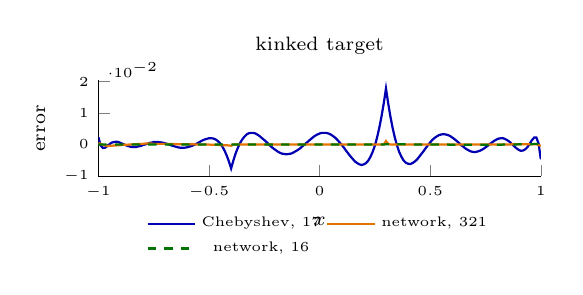
\begin{tikzpicture}
\begin{axis}[
    width=7.2cm, height=2.8cm,
    title={\scriptsize kinked target},
    xmin=-1, xmax=1, xlabel={\scriptsize $x$},
    ylabel={\scriptsize error},
    tick label style={font=\tiny}, label style={font=\tiny}, title style={font=\scriptsize},
    axis x line*=bottom, axis y line*=left,
    legend style={font=\tiny, draw=none, fill=none, at={(0.5,-0.30)}, anchor=north, legend columns=2}]
  \addplot[thick, blue!70!black] coordinates {(-1.0000,0.0023) (-0.9900,-0.0003) (-0.9800,-0.0011) (-0.9700,-0.0010) (-0.9600,-0.0005) (-0.9500,0.0001) (-0.9400,0.0006) (-0.9300,0.0008) (-0.9200,0.0009) (-0.9100,0.0008) (-0.9000,0.0005) (-0.8900,0.0002) (-0.8800,-0.0001) (-0.8700,-0.0004) (-0.8600,-0.0006) (-0.8500,-0.0008) (-0.8400,-0.0008) (-0.8300,-0.0008) (-0.8200,-0.0006) (-0.8100,-0.0005) (-0.8000,-0.0002) (-0.7900,0.0000) (-0.7800,0.0002) (-0.7700,0.0005) (-0.7600,0.0006) (-0.7500,0.0008) (-0.7400,0.0008) (-0.7300,0.0008) (-0.7200,0.0007) (-0.7100,0.0006) (-0.7000,0.0004) (-0.6900,0.0002) (-0.6800,-0.0000) (-0.6700,-0.0003) (-0.6600,-0.0005) (-0.6500,-0.0007) (-0.6400,-0.0009) (-0.6300,-0.0010) (-0.6200,-0.0010) (-0.6100,-0.0010) (-0.6000,-0.0009) (-0.5900,-0.0007) (-0.5800,-0.0005) (-0.5700,-0.0002) (-0.5600,0.0001) (-0.5500,0.0005) (-0.5400,0.0009) (-0.5300,0.0013) (-0.5200,0.0016) (-0.5100,0.0018) (-0.5000,0.0020) (-0.4900,0.0020) (-0.4800,0.0019) (-0.4700,0.0016) (-0.4600,0.0011) (-0.4500,0.0004) (-0.4400,-0.0006) (-0.4300,-0.0019) (-0.4200,-0.0035) (-0.4100,-0.0054) (-0.4000,-0.0076) (-0.3900,-0.0051) (-0.3800,-0.0029) (-0.3700,-0.0011) (-0.3600,0.0004) (-0.3500,0.0016) (-0.3400,0.0025) (-0.3300,0.0032) (-0.3200,0.0036) (-0.3100,0.0037) (-0.3000,0.0037) (-0.2900,0.0035) (-0.2800,0.0031) (-0.2700,0.0026) (-0.2600,0.0020) (-0.2500,0.0014) (-0.2400,0.0008) (-0.2300,0.0001) (-0.2200,-0.0006) (-0.2100,-0.0012) (-0.2000,-0.0017) (-0.1900,-0.0022) (-0.1800,-0.0026) (-0.1700,-0.0029) (-0.1600,-0.0030) (-0.1500,-0.0031) (-0.1400,-0.0030) (-0.1300,-0.0029) (-0.1200,-0.0026) (-0.1100,-0.0022) (-0.1000,-0.0018) (-0.0900,-0.0013) (-0.0800,-0.0007) (-0.0700,-0.0001) (-0.0600,0.0005) (-0.0500,0.0011) (-0.0400,0.0017) (-0.0300,0.0023) (-0.0200,0.0028) (-0.0100,0.0032) (0.0000,0.0035) (0.0100,0.0037) (0.0200,0.0037) (0.0300,0.0037) (0.0400,0.0035) (0.0500,0.0032) (0.0600,0.0027) (0.0700,0.0022) (0.0800,0.0015) (0.0900,0.0007) (0.1000,-0.0001) (0.1100,-0.0010) (0.1200,-0.0020) (0.1300,-0.0029) (0.1400,-0.0038) (0.1500,-0.0046) (0.1600,-0.0054) (0.1700,-0.0059) (0.1800,-0.0063) (0.1900,-0.0065) (0.2000,-0.0063) (0.2100,-0.0059) (0.2200,-0.0051) (0.2300,-0.0039) (0.2400,-0.0023) (0.2500,-0.0003) (0.2600,0.0023) (0.2700,0.0054) (0.2800,0.0090) (0.2900,0.0131) (0.3000,0.0178) (0.3100,0.0131) (0.3200,0.0089) (0.3300,0.0053) (0.3400,0.0022) (0.3500,-0.0003) (0.3600,-0.0024) (0.3700,-0.0039) (0.3800,-0.0051) (0.3900,-0.0058) (0.4000,-0.0061) (0.4100,-0.0062) (0.4200,-0.0059) (0.4300,-0.0054) (0.4400,-0.0048) (0.4500,-0.0039) (0.4600,-0.0030) (0.4700,-0.0021) (0.4800,-0.0011) (0.4900,-0.0002) (0.5000,0.0007) (0.5100,0.0015) (0.5200,0.0021) (0.5300,0.0026) (0.5400,0.0030) (0.5500,0.0032) (0.5600,0.0033) (0.5700,0.0032) (0.5800,0.0030) (0.5900,0.0027) (0.6000,0.0022) (0.6100,0.0017) (0.6200,0.0011) (0.6300,0.0005) (0.6400,-0.0002) (0.6500,-0.0007) (0.6600,-0.0013) (0.6700,-0.0017) (0.6800,-0.0021) (0.6900,-0.0023) (0.7000,-0.0024) (0.7100,-0.0023) (0.7200,-0.0021) (0.7300,-0.0018) (0.7400,-0.0014) (0.7500,-0.0009) (0.7600,-0.0004) (0.7700,0.0002) (0.7800,0.0007) (0.7900,0.0012) (0.8000,0.0016) (0.8100,0.0019) (0.8200,0.0020) (0.8300,0.0020) (0.8400,0.0017) (0.8500,0.0013) (0.8600,0.0008) (0.8700,0.0001) (0.8800,-0.0006) (0.8900,-0.0012) (0.9000,-0.0017) (0.9100,-0.0020) (0.9200,-0.0019) (0.9300,-0.0015) (0.9400,-0.0008) (0.9500,0.0003) (0.9600,0.0014) (0.9700,0.0022) (0.9800,0.0022) (0.9900,0.0003) (1.0000,-0.0047)};
  \addlegendentry{Chebyshev, 17}
  \addplot[thick, orange!90!black] coordinates {(-1.0000,0.0005) (-0.9900,0.0002) (-0.9800,-0.0001) (-0.9700,-0.0003) (-0.9600,-0.0005) (-0.9500,-0.0004) (-0.9400,-0.0004) (-0.9300,-0.0003) (-0.9200,-0.0003) (-0.9100,-0.0002) (-0.9000,-0.0002) (-0.8900,-0.0001) (-0.8800,-0.0001) (-0.8700,-0.0001) (-0.8600,-0.0000) (-0.8500,0.0000) (-0.8400,0.0001) (-0.8300,0.0001) (-0.8200,0.0002) (-0.8100,0.0002) (-0.8000,0.0002) (-0.7900,0.0003) (-0.7800,0.0003) (-0.7700,0.0003) (-0.7600,0.0003) (-0.7500,0.0002) (-0.7400,0.0002) (-0.7300,0.0002) (-0.7200,0.0002) (-0.7100,0.0002) (-0.7000,0.0002) (-0.6900,0.0002) (-0.6800,0.0002) (-0.6700,0.0002) (-0.6600,0.0002) (-0.6500,0.0001) (-0.6400,0.0001) (-0.6300,0.0001) (-0.6200,0.0001) (-0.6100,0.0001) (-0.6000,0.0001) (-0.5900,0.0001) (-0.5800,0.0001) (-0.5700,0.0001) (-0.5600,0.0000) (-0.5500,0.0000) (-0.5400,0.0000) (-0.5300,0.0000) (-0.5200,0.0000) (-0.5100,-0.0000) (-0.5000,-0.0000) (-0.4900,-0.0001) (-0.4800,-0.0001) (-0.4700,-0.0001) (-0.4600,-0.0001) (-0.4500,-0.0002) (-0.4400,-0.0002) (-0.4300,-0.0002) (-0.4200,-0.0002) (-0.4100,-0.0003) (-0.4000,-0.0004) (-0.3900,-0.0000) (-0.3800,-0.0000) (-0.3700,-0.0000) (-0.3600,-0.0000) (-0.3500,-0.0000) (-0.3400,-0.0000) (-0.3300,-0.0000) (-0.3200,-0.0000) (-0.3100,-0.0000) (-0.3000,-0.0000) (-0.2900,-0.0000) (-0.2800,-0.0000) (-0.2700,-0.0000) (-0.2600,-0.0000) (-0.2500,-0.0000) (-0.2400,-0.0000) (-0.2300,-0.0000) (-0.2200,-0.0000) (-0.2100,-0.0000) (-0.2000,-0.0000) (-0.1900,-0.0000) (-0.1800,-0.0000) (-0.1700,-0.0000) (-0.1600,-0.0000) (-0.1500,-0.0000) (-0.1400,-0.0000) (-0.1300,-0.0000) (-0.1200,-0.0000) (-0.1100,-0.0000) (-0.1000,-0.0000) (-0.0900,-0.0000) (-0.0800,-0.0000) (-0.0700,-0.0000) (-0.0600,-0.0000) (-0.0500,-0.0000) (-0.0400,-0.0000) (-0.0300,-0.0000) (-0.0200,-0.0000) (-0.0100,-0.0000) (0.0000,-0.0000) (0.0100,-0.0000) (0.0200,0.0000) (0.0300,0.0000) (0.0400,0.0000) (0.0500,0.0000) (0.0600,0.0000) (0.0700,0.0000) (0.0800,0.0000) (0.0900,0.0000) (0.1000,0.0000) (0.1100,0.0000) (0.1200,0.0000) (0.1300,0.0000) (0.1400,0.0000) (0.1500,0.0000) (0.1600,0.0000) (0.1700,0.0000) (0.1800,0.0000) (0.1900,0.0000) (0.2000,0.0000) (0.2100,0.0000) (0.2200,0.0000) (0.2300,0.0000) (0.2400,0.0000) (0.2500,0.0000) (0.2600,0.0000) (0.2700,0.0000) (0.2800,0.0000) (0.2900,0.0000) (0.3000,0.0011) (0.3100,0.0002) (0.3200,-0.0000) (0.3300,-0.0000) (0.3400,-0.0000) (0.3500,-0.0000) (0.3600,-0.0000) (0.3700,-0.0000) (0.3800,-0.0000) (0.3900,-0.0000) (0.4000,-0.0000) (0.4100,-0.0000) (0.4200,-0.0000) (0.4300,-0.0000) (0.4400,-0.0000) (0.4500,-0.0000) (0.4600,-0.0000) (0.4700,-0.0000) (0.4800,-0.0000) (0.4900,-0.0000) (0.5000,-0.0000) (0.5100,-0.0000) (0.5200,-0.0000) (0.5300,-0.0000) (0.5400,-0.0000) (0.5500,-0.0000) (0.5600,-0.0000) (0.5700,-0.0000) (0.5800,-0.0000) (0.5900,-0.0000) (0.6000,-0.0000) (0.6100,-0.0000) (0.6200,-0.0000) (0.6300,-0.0000) (0.6400,-0.0000) (0.6500,-0.0000) (0.6600,-0.0000) (0.6700,-0.0000) (0.6800,-0.0000) (0.6900,-0.0000) (0.7000,-0.0000) (0.7100,-0.0000) (0.7200,-0.0000) (0.7300,-0.0000) (0.7400,-0.0000) (0.7500,-0.0000) (0.7600,0.0000) (0.7700,0.0000) (0.7800,0.0000) (0.7900,0.0000) (0.8000,0.0000) (0.8100,0.0000) (0.8200,0.0000) (0.8300,0.0000) (0.8400,0.0000) (0.8500,0.0000) (0.8600,0.0000) (0.8700,0.0001) (0.8800,0.0001) (0.8900,0.0001) (0.9000,0.0001) (0.9100,0.0001) (0.9200,0.0001) (0.9300,0.0001) (0.9400,0.0001) (0.9500,0.0001) (0.9600,0.0001) (0.9700,0.0001) (0.9800,0.0001) (0.9900,-0.0002) (1.0000,-0.0004)};
  \addlegendentry{network, 321}
  \addplot[thick, green!45!black, dashed] coordinates {(-1.0000,-0.0000) (-0.9900,-0.0000) (-0.9800,-0.0000) (-0.9700,-0.0000) (-0.9600,-0.0000) (-0.9500,-0.0000) (-0.9400,-0.0000) (-0.9300,-0.0000) (-0.9200,-0.0000) (-0.9100,-0.0000) (-0.9000,-0.0000) (-0.8900,-0.0000) (-0.8800,-0.0000) (-0.8700,-0.0000) (-0.8600,-0.0000) (-0.8500,-0.0000) (-0.8400,-0.0000) (-0.8300,-0.0000) (-0.8200,-0.0000) (-0.8100,-0.0000) (-0.8000,-0.0000) (-0.7900,-0.0000) (-0.7800,-0.0000) (-0.7700,-0.0000) (-0.7600,-0.0000) (-0.7500,-0.0000) (-0.7400,-0.0000) (-0.7300,-0.0000) (-0.7200,-0.0000) (-0.7100,-0.0000) (-0.7000,-0.0000) (-0.6900,-0.0000) (-0.6800,-0.0000) (-0.6700,-0.0000) (-0.6600,-0.0000) (-0.6500,-0.0000) (-0.6400,-0.0000) (-0.6300,-0.0000) (-0.6200,-0.0000) (-0.6100,-0.0000) (-0.6000,-0.0000) (-0.5900,-0.0000) (-0.5800,-0.0000) (-0.5700,-0.0000) (-0.5600,-0.0000) (-0.5500,-0.0000) (-0.5400,-0.0000) (-0.5300,-0.0000) (-0.5200,-0.0000) (-0.5100,-0.0000) (-0.5000,-0.0000) (-0.4900,-0.0000) (-0.4800,-0.0000) (-0.4700,-0.0000) (-0.4600,-0.0000) (-0.4500,-0.0000) (-0.4400,-0.0000) (-0.4300,-0.0000) (-0.4200,-0.0000) (-0.4100,-0.0000) (-0.4000,-0.0000) (-0.3900,-0.0000) (-0.3800,-0.0000) (-0.3700,-0.0000) (-0.3600,-0.0000) (-0.3500,-0.0000) (-0.3400,-0.0000) (-0.3300,-0.0000) (-0.3200,-0.0000) (-0.3100,-0.0000) (-0.3000,-0.0000) (-0.2900,-0.0000) (-0.2800,-0.0000) (-0.2700,-0.0000) (-0.2600,-0.0000) (-0.2500,-0.0000) (-0.2400,-0.0000) (-0.2300,-0.0000) (-0.2200,-0.0000) (-0.2100,-0.0000) (-0.2000,-0.0000) (-0.1900,-0.0000) (-0.1800,-0.0000) (-0.1700,-0.0000) (-0.1600,-0.0000) (-0.1500,-0.0000) (-0.1400,-0.0000) (-0.1300,-0.0000) (-0.1200,-0.0000) (-0.1100,-0.0000) (-0.1000,-0.0000) (-0.0900,-0.0000) (-0.0800,-0.0000) (-0.0700,-0.0000) (-0.0600,-0.0000) (-0.0500,-0.0000) (-0.0400,-0.0000) (-0.0300,-0.0000) (-0.0200,-0.0000) (-0.0100,-0.0000) (0.0000,-0.0000) (0.0100,-0.0000) (0.0200,-0.0000) (0.0300,-0.0000) (0.0400,-0.0000) (0.0500,-0.0000) (0.0600,-0.0000) (0.0700,-0.0000) (0.0800,-0.0000) (0.0900,-0.0000) (0.1000,-0.0000) (0.1100,-0.0000) (0.1200,-0.0000) (0.1300,-0.0000) (0.1400,0.0000) (0.1500,0.0000) (0.1600,0.0000) (0.1700,0.0000) (0.1800,0.0000) (0.1900,0.0000) (0.2000,0.0000) (0.2100,0.0000) (0.2200,0.0000) (0.2300,0.0000) (0.2400,0.0000) (0.2500,0.0000) (0.2600,0.0000) (0.2700,0.0000) (0.2800,0.0000) (0.2900,0.0000) (0.3000,0.0001) (0.3100,0.0001) (0.3200,0.0001) (0.3300,0.0001) (0.3400,0.0001) (0.3500,0.0001) (0.3600,0.0001) (0.3700,0.0001) (0.3800,0.0001) (0.3900,0.0001) (0.4000,0.0001) (0.4100,0.0000) (0.4200,0.0000) (0.4300,0.0000) (0.4400,0.0000) (0.4500,0.0000) (0.4600,0.0000) (0.4700,0.0000) (0.4800,0.0000) (0.4900,0.0000) (0.5000,-0.0000) (0.5100,-0.0000) (0.5200,-0.0000) (0.5300,-0.0000) (0.5400,-0.0000) (0.5500,-0.0000) (0.5600,-0.0000) (0.5700,-0.0000) (0.5800,-0.0000) (0.5900,-0.0001) (0.6000,-0.0001) (0.6100,-0.0001) (0.6200,-0.0001) (0.6300,-0.0001) (0.6400,-0.0001) (0.6500,-0.0001) (0.6600,-0.0001) (0.6700,-0.0001) (0.6800,-0.0001) (0.6900,-0.0001) (0.7000,-0.0001) (0.7100,-0.0001) (0.7200,-0.0001) (0.7300,-0.0001) (0.7400,-0.0001) (0.7500,-0.0001) (0.7600,-0.0001) (0.7700,-0.0001) (0.7800,-0.0001) (0.7900,-0.0001) (0.8000,-0.0001) (0.8100,-0.0001) (0.8200,-0.0001) (0.8300,-0.0000) (0.8400,-0.0000) (0.8500,-0.0000) (0.8600,-0.0000) (0.8700,0.0000) (0.8800,0.0000) (0.8900,0.0000) (0.9000,0.0001) (0.9100,0.0001) (0.9200,0.0001) (0.9300,0.0001) (0.9400,0.0001) (0.9500,0.0001) (0.9600,0.0001) (0.9700,0.0002) (0.9800,0.0002) (0.9900,0.0002) (1.0000,0.0002)};
  \addlegendentry{network, 16}
\end{axis}
\end{tikzpicture}
\end{center}
\end{column}
\end{columns}
\vspace{-1mm}
\begin{center}\footnotesize
\begin{tabularx}{0.86\linewidth}{@{}>{\raggedright\arraybackslash}X >{\raggedright\arraybackslash}p{3.3cm} >{\raggedleft\arraybackslash}p{1.5cm} >{\raggedleft\arraybackslash}p{2.0cm}@{}}
\toprule
\textbf{Target} & \textbf{Method} & \textbf{Params} & \textbf{$\max|\text{err}|$} \\
\midrule
smooth & Chebyshev, degree $16$ & $17$ & $\mathbf{2.5\times10^{-11}}$ \\
smooth & network, $16$--$16$ & $321$ & $4.2\times10^{-2}$ \\
smooth & \textbf{network, $5$ --- matched} & $\mathbf{16}$ & $2.5\times10^{-1}$ \\
kinked & Chebyshev, degree $16$ & $17$ & $1.8\times10^{-2}$ \\
kinked & network, $16$--$16$ & $321$ & $1.1\times10^{-3}$ \\
kinked & \textbf{network, $5$ --- matched} & $\mathbf{16}$ & $\mathbf{2.0\times10^{-4}}$ \\
\bottomrule
\end{tabularx}
\end{center}
\vspace{1mm}
\src{Ledger \texttt{nn\_vs\_cheb}; deviation from the target, not the level. Code: \repo{tools/figures/s07_generate.py}{s07\_generate.py}, \texttt{run\_nn\_vs\_cheb}.}
\end{frame}

%=============================================================================
\begin{frame}{Read That Table Before You Believe Anything Else}
\begin{columns}[T]
\begin{column}{0.51\textwidth}
\small
\textbf{On the smooth function the network loses, badly.} Chebyshev with $17$ coefficients reaches $2.5\times10^{-11}$ --- machine precision. The network with $321$ parameters manages $4.2\times10^{-2}$: nineteen times the parameters and \textbf{nine orders of magnitude} worse. \textbf{Matched at $16$ parameters it is worse again}, $2.5\times10^{-1}$.
\medskip

\textbf{On the kinked function it wins outright.} Look at the right-hand panel: the Chebyshev error rings across the whole domain --- 5.B2's Gibbs phenomenon --- while the network's is flat.
\end{column}
\begin{column}{0.46\textwidth}
\begin{takeawaybox}[title=\textbf{The rule this gives you}]\footnotesize
\textbf{Smooth and low-dimensional} $\Rightarrow$ a spectral basis: faster, smaller, better. \textbf{Kinked, or high-dimensional} $\Rightarrow$ the adaptive basis earns its keep.
\end{takeawaybox}
\smallskip
\begin{cautionbox}[title=\textbf{``But the network had more parameters''}]\footnotesize
So the last row of each block matches it: \textbf{16 against 17}. Matched, the verdict sharpens both ways --- ten times worse on the smooth target, \textbf{$88\times$ better on the kinked one}, beating even the $321$-parameter net.
\end{cautionbox}
\end{column}
\end{columns}
\vspace{1mm}
\src{Kinks are not exotic in macroeconomics: a borrowing limit (2.A1), irreversible investment, a tax bracket, a zero lower bound.}
\end{frame}

%=============================================================================
\begin{frame}{Takeaways, and What Is Not Yet Settled}
\begin{columns}[T]
\begin{column}{0.55\textwidth}
\begin{takeawaybox}\small
\begin{itemize}\small\setlength{\itemsep}{1.1mm}
  \item A neuron is a regression with a nonlinear output; \textbf{without the nonlinearity, depth buys nothing at all}.
  \item Fix the kinks and a one-layer ReLU net \emph{is} least squares on a piecewise-linear basis. \textbf{Let them move and it finds the constraint}, at $1.0000$.
  \item Universal approximation is \textbf{existence}, not a recipe, and polynomials have it too.
  \item Barron's rate is free of $d$ \emph{in the exponent}; the dimension lives in $C_f$. \textbf{Theorem 6 is the sharp one:} a basis fixed in advance cannot beat $m^{-2/d}$.
  \item Measured: the network loses on a smooth target and wins on a kinked one.
\end{itemize}
\end{takeawaybox}
\end{column}
\begin{column}{0.42\textwidth}
\begin{conceptbox}[title=\textbf{Bridge to 7.A3}]\small
Every promise here was of the form ``a good network \emph{exists}''. Nothing has said how to find one.
\medskip
\textbf{7.A3 is the finding}: backpropagation, a first-order optimizer, and the discipline that keeps the fit honest. Including the $N=4$ row, which is what happens when the search does not deliver.
\end{conceptbox}
\end{column}
\end{columns}
\end{frame}

\end{document}
